\documentclass[../main.tex]{subfiles}
\usepackage{silence}
\WarningFilter{glossaries}{No \printglossary or \printglossaries found}
\robExtConfigure{disable externalization}
\begin{document}
\ifSubfilesClassLoaded{%
	\graphicspath{{figures/2-Background/}}%
	\setcounter{chapter}{1}%
	\mainmatter%
}{
	\graphicspath{{../figures/2-Background/}}%
}
\chapter{Background}\label{chap:background}
\minitocpagecentered

\section{Deep-Learning models}
	In this section, I will introduce the main deep learning architectures used for discriminative tasks: \glsxtrfull{mlp}, \glsxtrfull{cnn}, \glsxtrfull{gnn}.
	The work of this thesis relies on attention mechanisms.
	Therefore, I will detail the attention mechanism and its usage in the transformer architecture.
	I will also describe the \glsxtrfull{ae} and its probabilistic variant, the \glsxtrfull{vae}, as they are commonly used to study omics data.
	Finally, I will present the \glsxtrfull{gan} architecture, which is used in one project of this thesis.

	Let \(\symbf{x}\) be the input and \(y \in \left\{1,2, \ldots, C \right\} \) the associated label, where \(C\) is the number of classes.
	The dimension of \(\symbf{x}\) will be specified in each architecture described.
	For discriminative tasks, the goal is to return a prediction \(\hat{y} \in {\left[0,1\right]}^C\).
	The goal of the different deep learning architectures is to find the best approximation \(g^{*}\) that maps an input \(\symbf{x}\) into a class \(y\): \(y = g^{*}\left(\symbf{x}\right)\).
	A deep learning architecture defines a mapping \(y=g\left(\symbf{x}; \theta\right)\) and learns the parameters \(\theta\) that give the best function approximation.
	\vspace{-1\baselineskip}
	\subsection{\Glsfmtfull{mlp}}\label{subsec:mlp}
		\begin{wrapfigure}[12]{O}{0.4\textwidth}
			\vspace{-1\intextsep}
			\centering
			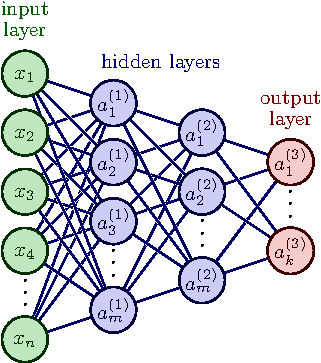
\includegraphics{mlp.pdf}
			\caption{Architecture of an \glsfmtshort{mlp}}\label{fig:mlp}
		\end{wrapfigure}
		\Gls{mlp} is an architecture taking one-dimensional input, \(\symbf{x} \in \symbb{R}^d\).
		The architecture comprises an input layer, \(L\) hidden layers, and one output layer.
		There are a total of \(L+2\) layers, \(L=0\) corresponds to the input layer, and the layer \(L+1\) is the output layer.
		The input layer has \(d\) neurons, one for each input feature in \(\symbf{x}\).
		The number of neurons in the output layer depends on the type of task:
		\begin{itemize}[nosep, topsep=-5pt]
			\item for binary classification, \(C=2\), it has only one neuron,
			\item for multiclass classification \(C > 2 \), it has one neuron per class.
		\end{itemize}
		Each hidden layer \(l\) has a defined number of neurons \(N_{l}\).
		Each neuron \(j\) in a layer \(l\) is connected to all neurons in the layer \(l-1\).
		Connection between a neuron \(i\) in layer \(l-1\) and neuron \(j\) in layer \(l\) is weighted by \(w^{l}_{ij}\).

		The activation of a neuron \(j\) in layer \(l\) is the non-linear activation \(f\) of the weighted-sum of neurons in layer \(l-1\) and some bias \(b_{j}^{l}\)~(\cref{eq:mlp_neuron}).
		\begin{align}
			a_{j}^{l} & = f\left(\sum_{i}^{N_{l-1}}a_{i}^{l-1}w_{ij}^{l} + b_{j}^{l} \right) \\ \label{eq:mlp_neuron}
			          & = f\left(z^{l}\right)
		\end{align}
		The computation of the activation of all neurons in layer \(l\) can be expressed in a matrix form:
		\begin{equation}
			\symbf{a}^{l} = f\left( \symbf{a}^{l-1} \cdot W^l + \symbf{b}^{l} \right) \label{eq:mlp_matrix}
		\end{equation}
		where \(W^l \in \symbb{R}^{N_{l-1} \times N_{l}}\) is the weight matrix of general element: \(w_{ij}\), and \(\symbf{b}^{l}\) is the bias vector of layer \(l\).
		The non-linear activation \(f\) is usually a \glsxtrfull{relu}, \(f\left(x\right) = \max\left(0, x\right)\)~\cite{ReluRef}.
		The activation of neurons in layers \(l\)~(\cref{eq:mlp_matrix}) defines a mapping \(g^{l}\) that computes the activation of layer \(l\) from the activation of layer \(l-1\): \( \symbf{a}^{l} = g^{l}\left(\symbf{a}^{l-1}; \theta^{l}\right)\), where \(\theta^{l}\) are the parameters of the layer \(l\): \(W^l\) and \( \symbf{b}^{l}\).
		This type of layer is called a \glsxtrfull{fcl} or dense layer.
		The composition of multiple \glspl{fcl} is called a \glsxtrfull{fcn}.
		The activation function of the last layer, layer \(L+1\), depends on the type of task:
		\begin{itemize}
			\item for binary classification, the unique output neuron has a sigmoid activation: \(a^{L+1} = \cfrac{1}{1-\exp\left(z^{L+1}\right)}\) and yields the probability of the positive class,
			\item for multiclass classification, a softmax activation function is used: \(a_{c}^{L} = \cfrac{\exp\left(z_{c}^{L+1}\right)}{\sum_{j}^{C}\exp\left(z_{j}^{L+1}\right)}\), each \(a_{c}^{L}\) gives the probability that the input \(\symbf{x}\) belongs to the class \(c\).
		\end{itemize}
		The mapping \(g\) of the \gls{mlp} can be expressed as the composition of the mapping of the individual layer: \(g = g^{L+1} \circ g^{L} \circ \cdots \circ g^{1}\).

		\Gls{mlp} are called feedforward networks; the information flows from the input \(\symbf{x}\) to the output \(y\) without any feedback connection, where the output of the model would be fed back to the model itself.

		The \gls{mlp} is one of the simplest models but can have many parameters, especially for high-dimensional inputs.
		Indeed, the number of parameters roughly corresponds to the sum of the number of parameters in each weight matrix \(W^{l}\).
		The weight matrix \(W^1\) depends on the input dimension \(d\); the larger \(d\), the higher the number of parameters to learn.

	\subsection{\Glsfmtfull{cnn}}
		\Gls{cnn} is an architecture composed of an input layer, \(L\) hidden layers and one output layer.
		This architecture has been initially developed for images; hence it accepts three-dimensional inputs \(\symbf{x} \in \symbb{R}^{h\times w \times p} \), where \(h\), \(w\) are respectively the height and the width of the image.
		\(p\) represents the number of channels; a gray image has only one channel, whereas an RGB image has three channels.
		Compared to the \gls{mlp}, some hidden layers are replaced with convolutional and pooling layers.
		Convolution layers are based on the convolution of a one-channel input with a two-dimensional kernel \(K\)~(\cref{eq:conv}).
		\begin{equation}
			\left(K * \symbf{x}\right)\left(i,j\right) =\sum_m\sum_n \symbf{x}_{i-m, j-n}K_{m,n} \label{eq:conv}
		\end{equation}
		Usually, multiple filters are applied simultaneously to the multiple input channels.
		In this case, the kernel is four-dimensional to account for the in and out channels dimensions~(\cref{eq:conv_multi}).
		\begin{equation}
			\left(K * \symbf{x}\right)\left(i,j, c_{out}\right) =\sum_m\sum_n \symbf{x}_{i-m, j-n, c_{in}}K_{m,n, c_{in}, c_{out}} \label{eq:conv_multi}
		\end{equation}
		After convolving the inputs, a bias term is added, and a \gls{relu} activation is applied.
		After one or more convolution layers, a pooling layer is used to introduce some invariance by combining the neurons in the fixed window to a single neuron in the next layer.
		The neurons in the window are usually reduced with the maximum or average function.
		The output layer is similar to the one used with the \gls{mlp}; for binary classification, a single neuron with a sigmoid activation is used, and for multiclass classification problems, there is one neuron per class with a softmax activation~(\cref{subsec:mlp}).

		Similarly to \glspl{mlp}, \glspl{cnn} are feedforward networks, the mapping \(g\) of the \gls{cnn} is also expressed as the composition of the mapping of the individual layers.

		As the \gls{cnn} is constructed around the convolution operator, it can easily be adapted to use one-dimensional input, \(\symbf{x} \in \symbb{R}^d\), by using one-dimensional kernel instead of two-dimensional kernel.
		It should be noted that using the convolution operator implies spatial dependencies between input features.

	\subsection{\Glsfmtfull{gnn}}
		\Gls{gnn} is an architecture that processes graphs~\cite{GNNRefs}.
		A graph \(\symcal{G}\) is a structure that consists of vertices \(\symcal{V}\) and edges \(\symcal{E}\).
		An edge \(\left(u,v\right) \in \symcal{V}^2,\, u\neq v\) connects two vertices \(u\) and \(v\), this link represents a relationship between the two vertices.
		The relationship between two nodes can be directed or undirected.
		In a homogeneous graph, each vertex represents the same type of entities, whereas, in a heterogeneous graph, each node can represent different types of entities.
		When different relationship types exist between two nodes, the graph is called a multigraph.
		Graphs are ubiquitous and are found in many domains:
		\begin{itemize}[nosep]
			\item molecules are graphs where nodes represent an atom and edges the covalent bond between two atoms,
			\item social networks are graphs where nodes represent people and edges a relationship between two people,
			\item the scientific literature can be seen as a graph, nodes represent a paper and edges a citation,
			\item in biology \gls{ppi} networks are graphs where nodes represent a protein and edges describe an interaction between two proteins.
		\end{itemize}

		A graph is represented by three different matrices: its adjacency matrix \(A \in {\left\{0,1\right\}}^{\left|\symcal{V}\right| \times \left|\symcal{V}\right|}\) which describe the structure of the graph, the node embeddings \(X \in \symbb{R}^{\left|\symcal{V}\right| \times d_v}\) and the edge embeddings \(E \in \symbb{R}^{\left|\symcal{V}\right| \times d_e}\).
		Each row of the node embedding matrix, \(X_{v}\), is node \(v\) \(d_v\)-length vector embedding.
		Similarly, each row of the edge embeddings matrix is the \(d_e\)-length vector embedding of an edge.
		In the following, I will focus on undirected graphs without edge embedding \(E\).

		\begin{figure}[htbp]
			\centering
			\ifSubfilesClassLoaded{%
				\begin{tikzpicture}

    \node[draw, circle, thick, inner sep=1pt, font=\scriptsize, minimum size=1.2em, fill=orange!70] (n1) at (0,0) {1};
    \node[draw, circle, thick, inner sep=1pt, font=\scriptsize, minimum size=1.2em, fill=blue!80] (n2) at (1,0) {2};
    \node[draw, circle, thick, inner sep=1pt, font=\scriptsize, minimum size=1.2em, fill=violet!70] (n3) at (1.5,0.75) {3};
    \node[draw, circle, thick, inner sep=1pt, font=\scriptsize, minimum size=1.2em, fill=teal!70] (n4) at (1.1,-0.9) {4};
    \node[draw, circle, thick, inner sep=1pt, font=\scriptsize, minimum size=1.2em, fill=magenta!70] (n5) at (0.5,0.75) {5};
    \node[draw, circle, thick, inner sep=1pt, font=\scriptsize, minimum size=1.2em, fill=blue!50] (n6) at (-0.3,-0.75) {6};
    \node[draw, circle, thick, inner sep=1pt, font=\scriptsize, minimum size=1.2em, fill=red!80] (n7) at (-1.2,-0.75) {7};
    \node[draw, circle, thick, inner sep=1pt, font=\scriptsize, minimum size=1.2em, fill=cyan!70] (n8) at (-0.75,0.75) {8};
    \node[draw, circle, thick, inner sep=1pt, font=\scriptsize, minimum size=1.2em, fill=purple!80] (n9) at (-1.8,1) {9};
    \node[draw, circle, thick, inner sep=1pt, font=\scriptsize, minimum size=1.2em, fill=yellow!70] (n10) at (-1.5,0.2) {10};
    \node (glab) [inner sep=1pt, font=\mathversion{smaller}] at (-2.1,0.2) {\(\symcal{G}\)};

    \draw[thick] (n1) -- (n2);
    \draw[thick] (n3) -- (n2);
    \draw[thick] (n4) -- (n2);
    \draw[thick] (n1) -- (n5);
    \draw[thick] (n1) -- (n6);
    \draw[thick] (n7) -- (n6);
    \draw[thick] (n1) -- (n8);
    \draw[thick] (n9) -- (n8);
    \draw[thick] (n10) -- (n8);

    \draw[-stealth, very thick] (1.3,0) -- (2.4,0);
    \draw[-stealth, very thick] (1.8,-2.2) -- (2.4,-2.2);
    \begin{scope}[yshift=-3.6cm, xshift=-1.5cm]
        \fill[orange!70, inner sep=0pt] (0,1.8) rectangle (3,2);
        \fill[blue!80, inner sep=0pt] (0,1.6) rectangle (3,1.8);
        \fill[violet!70, inner sep=0pt] (0,1.4) rectangle (3,1.6);
        \fill[teal!70, inner sep=0pt] (0,1.2) rectangle (3,1.4);
        \fill[magenta!70, inner sep=0pt] (0,1) rectangle (3,1.2);
        \fill[blue!50, inner sep=0pt] (0,0.8) rectangle (3,1);
        \fill[red!80, inner sep=0pt] (0,0.6) rectangle (3,0.8);
        \fill[cyan!70, inner sep=0pt] (0,0.4) rectangle (3,0.6);
        \fill[purple!80, inner sep=0pt] (0,0.2) rectangle (3,0.4);
        \fill[yellow!70, inner sep=0pt] (0,0) rectangle (3,0.2);
        \draw[step=2mm, black] (0,0) grid (3,2);
        \draw[black,thick] (0,0) rectangle (3,2);
        \draw[stealth-stealth] ([xshift=3pt]3,0) -- node [midway, anchor=west, font=\mathversion{middlesize}, inner sep=1pt] {\(\left|\symcal{V}\right|\)} ([xshift=3pt]3,2);
        \draw[stealth-stealth] ([yshift=3pt]0,2) -- node [midway, anchor=south, font=\mathversion{middlesize}, inner sep=1pt] {\(d_{v}\)} ([yshift=3pt]3,2);
        \coordinate (xpos) at (0,1);
        \node[font=\mathversion{middlesize}, anchor=center, inner sep=2pt] at (glab.south |- xpos.west) {\(X\)};


    \end{scope}

    \draw[black,thick, rounded corners=5, fill=pink!60] (2.5,-3) rectangle (3,1);
    \node (GCN1) [rotate=90,font=\mathversion{smaller}] at (2.75,-1) {\(\operatorname{GCN}\)};
    \node (relu1) [right=5mm of GCN1.south, anchor=north, draw, rounded corners=5,font=\mathversion{smaller}, rotate=90, thick, fill=red!70] {\(\operatorname{ReLU}\)};
    \draw[black,thick, rounded corners=5, fill=pink!60] (4.7,-3) rectangle (5.2,1);
    \node (GCN2) [rotate=90,font=\mathversion{smaller}] at (4.95,-1) {\(\operatorname{GCN}\)};
    \node (relu_last) [right=5mm of GCN2.south, anchor=north, draw, rounded corners=5,font=\mathversion{smaller}, rotate=90, thick, fill=red!70] {\(\operatorname{ReLU}\)};
    \node (readout) [right=5mm of relu_last.south, anchor=north, draw, rounded corners=5,font=\footnotesize, rotate=90, thick, fill=purple!40] {Readout};
    \node (fcn) [right=5mm of readout.south, anchor=north, draw, rounded corners=5,font=\mathversion{smaller}, rotate=90, thick, fill=cyan!50] {\(\operatorname{FCN}\)};
    \node (preds) [right=5mm of fcn.south, anchor=west, draw, rounded corners=5,font=\mathversion{smaller}, thick] {\(\hat{y}\)};

    \draw[-stealth, thick] (GCN1.south) -- (relu1.north);
    \draw[-stealth, thick] (relu1.south) -- (GCN2.north);
    \draw[-stealth, thick] (GCN2.south) -- (relu_last.north);
    \draw[-stealth, thick] (relu_last.south) -- (readout.north);
    \draw[-stealth, thick] (readout.south) -- (fcn.north);
    \draw[-stealth, thick] (fcn.south) -- (preds.west);

    %\node[fit={(GCN1)(preds)}, draw, ultra thick, rounded corners, inner ysep=1.5cm] (gnn) {};

    \begin{scope}[yshift=-5cm, xshift=0cm]
        \node[draw, circle, thick, inner sep=1pt, font=\scriptsize, minimum size=1.2em, fill=orange!70] (n1) at (0,0) {1};
        \node[draw, circle, thick, inner sep=1pt, font=\scriptsize, minimum size=1.2em, fill=blue!80] (n2) at (1,0) {2};
        \node[draw, circle, thick, inner sep=1pt, font=\scriptsize, minimum size=1.2em, fill=violet!70] (n3) at (1.5,0.75) {3};
        \node[draw, circle, thick, inner sep=1pt, font=\scriptsize, minimum size=1.2em, fill=teal!70] (n4) at (1.1,-0.9) {4};
        \draw[thick] (n1) -- (n2);
        \draw[thick] (n3) -- (n2);
        \draw[thick] (n4) -- (n2);
        \node (eq) [font=\mathversion{smaller}, anchor=west] at (2.3,0) {\(\textcolor{blue!80}{h_{2}} = \textcolor{red!70}{f}\left(\cfrac{\textcolor{blue!80}{h_{2}}W}{3} + \cfrac{\left(\textcolor{violet!70}{h_{3}} + \textcolor{teal!70}{h_{4}}\right)W}{\sqrt{3}}+ \cfrac{\textcolor{orange!70}{h_{1}}W}{\sqrt{12}}\right)\)};
        \node[fit={(n1)(n4)(eq)(n3)}, draw, ultra thick, rounded corners] (gconvdetails) {};
        \node (gcnlabel) [draw, very thick, rounded corners, anchor=center, inner sep=3pt, fill=white, font=\footnotesize] at (gconvdetails.north) {Graph convolution on node 2};

    \end{scope}
    \draw[dashed, thick] (4.7,-3) -- (gcnlabel.north west);
    \draw[dashed, thick] (5.2,-3) -- (gcnlabel.north east);
\end{tikzpicture}%
			}{
				\begin{tikzpicture}

    \node[draw, circle, thick, inner sep=1pt, font=\scriptsize, minimum size=1.2em, fill=orange!70] (n1) at (0,0) {1};
    \node[draw, circle, thick, inner sep=1pt, font=\scriptsize, minimum size=1.2em, fill=blue!80] (n2) at (1,0) {2};
    \node[draw, circle, thick, inner sep=1pt, font=\scriptsize, minimum size=1.2em, fill=violet!70] (n3) at (1.5,0.75) {3};
    \node[draw, circle, thick, inner sep=1pt, font=\scriptsize, minimum size=1.2em, fill=teal!70] (n4) at (1.1,-0.9) {4};
    \node[draw, circle, thick, inner sep=1pt, font=\scriptsize, minimum size=1.2em, fill=magenta!70] (n5) at (0.5,0.75) {5};
    \node[draw, circle, thick, inner sep=1pt, font=\scriptsize, minimum size=1.2em, fill=blue!50] (n6) at (-0.3,-0.75) {6};
    \node[draw, circle, thick, inner sep=1pt, font=\scriptsize, minimum size=1.2em, fill=red!80] (n7) at (-1.2,-0.75) {7};
    \node[draw, circle, thick, inner sep=1pt, font=\scriptsize, minimum size=1.2em, fill=cyan!70] (n8) at (-0.75,0.75) {8};
    \node[draw, circle, thick, inner sep=1pt, font=\scriptsize, minimum size=1.2em, fill=purple!80] (n9) at (-1.8,1) {9};
    \node[draw, circle, thick, inner sep=1pt, font=\scriptsize, minimum size=1.2em, fill=yellow!70] (n10) at (-1.5,0.2) {10};
    \node (glab) [inner sep=1pt, font=\mathversion{smaller}] at (-2.1,0.2) {\(\symcal{G}\)};

    \draw[thick] (n1) -- (n2);
    \draw[thick] (n3) -- (n2);
    \draw[thick] (n4) -- (n2);
    \draw[thick] (n1) -- (n5);
    \draw[thick] (n1) -- (n6);
    \draw[thick] (n7) -- (n6);
    \draw[thick] (n1) -- (n8);
    \draw[thick] (n9) -- (n8);
    \draw[thick] (n10) -- (n8);

    \draw[-stealth, very thick] (1.3,0) -- (2.4,0);
    \draw[-stealth, very thick] (1.8,-2.2) -- (2.4,-2.2);
    \begin{scope}[yshift=-3.6cm, xshift=-1.5cm]
        \fill[orange!70, inner sep=0pt] (0,1.8) rectangle (3,2);
        \fill[blue!80, inner sep=0pt] (0,1.6) rectangle (3,1.8);
        \fill[violet!70, inner sep=0pt] (0,1.4) rectangle (3,1.6);
        \fill[teal!70, inner sep=0pt] (0,1.2) rectangle (3,1.4);
        \fill[magenta!70, inner sep=0pt] (0,1) rectangle (3,1.2);
        \fill[blue!50, inner sep=0pt] (0,0.8) rectangle (3,1);
        \fill[red!80, inner sep=0pt] (0,0.6) rectangle (3,0.8);
        \fill[cyan!70, inner sep=0pt] (0,0.4) rectangle (3,0.6);
        \fill[purple!80, inner sep=0pt] (0,0.2) rectangle (3,0.4);
        \fill[yellow!70, inner sep=0pt] (0,0) rectangle (3,0.2);
        \draw[step=2mm, black] (0,0) grid (3,2);
        \draw[black,thick] (0,0) rectangle (3,2);
        \draw[stealth-stealth] ([xshift=3pt]3,0) -- node [midway, anchor=west, font=\mathversion{middlesize}, inner sep=1pt] {\(\left|\symcal{V}\right|\)} ([xshift=3pt]3,2);
        \draw[stealth-stealth] ([yshift=3pt]0,2) -- node [midway, anchor=south, font=\mathversion{middlesize}, inner sep=1pt] {\(d_{v}\)} ([yshift=3pt]3,2);
        \coordinate (xpos) at (0,1);
        \node[font=\mathversion{middlesize}, anchor=center, inner sep=2pt] at (glab.south |- xpos.west) {\(X\)};


    \end{scope}

    \draw[black,thick, rounded corners=5, fill=pink!60] (2.5,-3) rectangle (3,1);
    \node (GCN1) [rotate=90,font=\mathversion{smaller}] at (2.75,-1) {\(\operatorname{GCN}\)};
    \node (relu1) [right=5mm of GCN1.south, anchor=north, draw, rounded corners=5,font=\mathversion{smaller}, rotate=90, thick, fill=red!70] {\(\operatorname{ReLU}\)};
    \draw[black,thick, rounded corners=5, fill=pink!60] (4.7,-3) rectangle (5.2,1);
    \node (GCN2) [rotate=90,font=\mathversion{smaller}] at (4.95,-1) {\(\operatorname{GCN}\)};
    \node (relu_last) [right=5mm of GCN2.south, anchor=north, draw, rounded corners=5,font=\mathversion{smaller}, rotate=90, thick, fill=red!70] {\(\operatorname{ReLU}\)};
    \node (readout) [right=5mm of relu_last.south, anchor=north, draw, rounded corners=5,font=\footnotesize, rotate=90, thick, fill=purple!40] {Readout};
    \node (fcn) [right=5mm of readout.south, anchor=north, draw, rounded corners=5,font=\mathversion{smaller}, rotate=90, thick, fill=cyan!50] {\(\operatorname{FCN}\)};
    \node (preds) [right=5mm of fcn.south, anchor=west, draw, rounded corners=5,font=\mathversion{smaller}, thick] {\(\hat{y}\)};

    \draw[-stealth, thick] (GCN1.south) -- (relu1.north);
    \draw[-stealth, thick] (relu1.south) -- (GCN2.north);
    \draw[-stealth, thick] (GCN2.south) -- (relu_last.north);
    \draw[-stealth, thick] (relu_last.south) -- (readout.north);
    \draw[-stealth, thick] (readout.south) -- (fcn.north);
    \draw[-stealth, thick] (fcn.south) -- (preds.west);

    %\node[fit={(GCN1)(preds)}, draw, ultra thick, rounded corners, inner ysep=1.5cm] (gnn) {};

    \begin{scope}[yshift=-5cm, xshift=0cm]
        \node[draw, circle, thick, inner sep=1pt, font=\scriptsize, minimum size=1.2em, fill=orange!70] (n1) at (0,0) {1};
        \node[draw, circle, thick, inner sep=1pt, font=\scriptsize, minimum size=1.2em, fill=blue!80] (n2) at (1,0) {2};
        \node[draw, circle, thick, inner sep=1pt, font=\scriptsize, minimum size=1.2em, fill=violet!70] (n3) at (1.5,0.75) {3};
        \node[draw, circle, thick, inner sep=1pt, font=\scriptsize, minimum size=1.2em, fill=teal!70] (n4) at (1.1,-0.9) {4};
        \draw[thick] (n1) -- (n2);
        \draw[thick] (n3) -- (n2);
        \draw[thick] (n4) -- (n2);
        \node (eq) [font=\mathversion{smaller}, anchor=west] at (2.3,0) {\(\textcolor{blue!80}{h_{2}} = \textcolor{red!70}{f}\left(\cfrac{\textcolor{blue!80}{h_{2}}W}{3} + \cfrac{\left(\textcolor{violet!70}{h_{3}} + \textcolor{teal!70}{h_{4}}\right)W}{\sqrt{3}}+ \cfrac{\textcolor{orange!70}{h_{1}}W}{\sqrt{12}}\right)\)};
        \node[fit={(n1)(n4)(eq)(n3)}, draw, ultra thick, rounded corners] (gconvdetails) {};
        \node (gcnlabel) [draw, very thick, rounded corners, anchor=center, inner sep=3pt, fill=white, font=\footnotesize] at (gconvdetails.north) {Graph convolution on node 2};

    \end{scope}
    \draw[dashed, thick] (4.7,-3) -- (gcnlabel.north west);
    \draw[dashed, thick] (5.2,-3) -- (gcnlabel.north east);
\end{tikzpicture}%
			}
			\caption[Example of a \glsfmtlong{gnn}]{Example of a \glsfmtlong{gnn} with two graph convolution layers. The details of the computation of the graph convolution for the node 2 is given. }\label{fig:gnn}
		\end{figure}

		A \gls{gnn} is an architecture composed of an input layer, \(L\) hidden layers, and one output layer.
		Similarly to the \gls{cnn}, some hidden layers are replaced with graph convolution layers
		\Glspl{gcn}, update node embeddings by aggregating information from neighboring nodes.
		The embedding of node \(v\), \(h^{l+1}_{v} \in \symbb{R}^{d_{l+1}}\) is updated by combining its previous embedding \(h^{l}_{v} \in \symbb{R}^{d_{l}}\) with the aggregated embedding \(h^{l}_{v,\text{agg}}\) from neighboring nodes \(\symcal{N}_{v}\):
		\begin{align}
			h^{l+1}_{v}          & = f\left( \frac{h^{l}_{v}W^{l}}{\left|\symcal{N}_{v} \right|} + h^{l}_{v,\text{agg}}W^{l}\right)                \\
			h^{l}_{v,\text{agg}} & = \sum_{u \in \symcal{N}_{v}} \frac{h^{l}_{u}}{\sqrt{\left|\symcal{N}_{v} \right|\left|\symcal{N}_{u} \right|}}
		\end{align}
		The weight \(W^{l} \in \symbb{R}^{d_{l}\times d_{l+1}}\) is the learnable weight matrix applied to the node embeddings, and \(f\) is a non-linear activation function, such as \(\operatorname{ReLU}\).
		Node embeddings \(h_{u}^{l}\) are normalized by the size of their neighborhood, \ie{}their degree: \(\left|\symcal{N}_{u} \right|\) to prevent explosion of the embeddings.
		The updates of all nodes can be written in the following matrix form:
		\begin{equation}
			H_{l+1} = \tilde{D}^{-\tfrac12}\tilde{A}\tilde{D}^{-\tfrac12}H_{l}W^{l}
		\end{equation}
		where, \(\tilde{A} = A + I_{\left|\symcal{V}\right|}\) is the adjacency matrix with self loops added, \(\tilde{D}\) is the corresponding degree matrix, and \(H_{l} \in \symbb{R}^{\left|\symcal{V}\right| \times d_{l}}\) is the node embedding matrix at layer \(l\).
		Variations of the aggregation step have been proposed; for instance, graph attention network~\cite{velickovic2018graph} weight the neighborhood based on attention mechanism or spectral approaches where the aggregation is done in the Fourier space~\cite{ChebConv}.

		With \glspl{gnn}, predictions can be made at different levels:
		\begin{itemize}[nosep]
			\item \textbf{Graph level}: The model outputs a prediction for the entire graph.
				The different node embeddings are combined before passing to a classifier network, often a \gls{mlp}.
			\item \textbf{Node level}: The model makes a prediction for each node individually.
				Each node embedding is passed to a classifier network.
			\item \textbf{Edge level}: predict the existence of an edge between two nodes.
		\end{itemize}

	\subsection{Self-attention and transformers}\label{sec:self_attention_transformer}

		\begin{figure}[htbp]
			\centering
			\begin{subcaptiongroup}
				\ifSubfilesClassLoaded{%
					\begin{tikzpicture}[
        module/.style={draw, very thick, rounded corners, minimum width=10ex},
        embmodule/.style={module, fill=red!40},
        mhamodule/.style={module, fill=orange!40},
        lnmodule/.style={module, fill=yellow!40},
        ffnmodule/.style={module, fill=cyan!40},
        arrow/.style={-stealth, thick, rounded corners},
    ]
    \begin{scope}[local bounding box=transBlock]
        \node[embmodule] (inputemb) {\(X\)};

        \node[above=of inputemb, mhamodule, align=center] (mha) {\(\operatorname{MHSA}\)};
        \node (add) [draw, thick, fill=white, circle, minimum size=2ex, above=5mm of mha.north, anchor=center] {};
        \draw[thick] (add.west) -- (add.east);
        \draw[thick] (add.north) -- (add.south);
        \node[above=of mha, lnmodule, align=center] (addnorm1) {\(\operatorname{LN}\)};
        \node[above=8mm of addnorm1, ffnmodule, align=center] (ffn) {\(\operatorname{FFN}\)};
        \node (add2) [draw, thick, fill=white, circle, minimum size=2ex, above=5mm of ffn.north, anchor=center] {};
        \draw[thick] (add2.west) -- (add2.east);
        \draw[thick] (add2.north) -- (add2.south);
        \node[above=of ffn, lnmodule, align=center] (addnorm2) {\(\operatorname{LN}\)};
        \node[above=5mm of addnorm2] (outputs) {};

        \coordinate (mharesidual) at ($(mha.south)!0.5!(inputemb.north)$);
        \coordinate (ffnresidual) at ($(ffn.south)!0.5!(addnorm1.north)$);
        \coordinate (mhafork) at ($(mha.south)!0.7!(mharesidual)$);
        \coordinate[left=5ex of add] (ln1residualleft);
        \coordinate[left=5ex of add2] (ln2residualleft);

        \node[fit={(mha)(addnorm2)(mharesidual)(ln1residualleft)}, draw, ultra thick, rounded corners] (encoder) {};
        \node[rotate=90, anchor=south] at (encoder.west) {\(\operatorname{TransformerBlock}\)};
        \node[anchor=south east, font=\bfseries, inner sep=2pt] at (encoder.north west) {A};


        \draw[arrow] (inputemb) -- (mha);
        \draw[arrow] (mha) -- (addnorm1);
        \draw[arrow] (addnorm1) -- (ffn);
        \draw[arrow] (ffn) -- (addnorm2);
        \draw[arrow] (addnorm2) -- (outputs);

        \draw[arrow] (mharesidual)-|(ln1residualleft)--(add);
        \draw[arrow] (ffnresidual)-|(ln2residualleft)--(add2);
        \draw[arrow] (mhafork)-|($(mha.south)!0.5!(mha.south west)$);
        \draw[arrow] (mhafork)-|($(mha.south)!0.5!(mha.south east)$);
    \end{scope}

    \begin{scope}[shift={($(transBlock.east)+(1.77cm,-2.35cm)$)}, local bounding box=mhsaBlock]
        \node (query) at (0,0) [inner sep =2pt,embmodule, minimum size=2.5ex] {\(X\)};

        \node (lin1) at (0,0) [draw, fill=cyan!40, thick, rectangle, rounded corners=5, copy shadow={opacity=.6, shadow xshift=0.7ex,shadow yshift=0.7ex}, above=5mm of query.north, anchor=south, minimum height=4ex,font=\mathversion{smaller}] {\(W_{1}^{Q}\)};
        \node (lin1) at (0,0) [draw, fill=cyan!40, thick, rectangle, rounded corners=5, copy shadow={opacity=.3, shadow xshift=1.4ex,shadow yshift=1.4ex}, above=5mm of query.north, anchor=south, minimum height=4ex,font=\mathversion{smaller}] {\(W_{1}^{Q}\)};

        \node (lin2) at (0,0) [draw, fill=cyan!40, thick, rectangle, rounded corners=5, copy shadow={opacity=.6, shadow xshift=0.7ex,shadow yshift=0.7ex}, right=5mm of lin1.east, anchor=west, minimum height=4ex,font=\mathversion{smaller}] {\(W_{1}^{K}\)};
        \node (lin2) at (0,0) [draw, fill=cyan!40, thick, rectangle, rounded corners=5, copy shadow={opacity=.3, shadow xshift=1.4ex,shadow yshift=1.4ex}, right=5mm of lin1.east, anchor=west, minimum height=4ex,font=\mathversion{smaller}] {\(W_{1}^{K}\)};

        \node (lin3) at (0,0) [draw, fill=cyan!40, thick, rectangle, rounded corners=5, copy shadow={opacity=.6, shadow xshift=0.7ex,shadow yshift=0.7ex}, right=5mm of lin2.east, anchor=west, minimum height=4ex,font=\mathversion{smaller}] {\(W_{1}^{V}\)};
        \node (lin3) at (0,0) [draw, fill=cyan!40, thick, rectangle, rounded corners=5, copy shadow={opacity=.3, shadow xshift=1.4ex,shadow yshift=1.4ex}, right=5mm of lin2.east, anchor=west, minimum height=4ex,font=\mathversion{smaller}] {\(W_{1}^{V}\)};

        \node (key) at (0,0) [inner sep =2pt,embmodule, minimum size=2.5ex,below=5mm of lin2.south, anchor=north] {\( X\)};
        \node (val) at (0,0) [inner sep =2pt,embmodule, minimum size=2.5ex, below=5mm of lin3.south, anchor=north] {\( X\)};

        \draw[thick, -stealth] (query.north) -- (lin1.south);
        \draw[thick, -stealth, opacity=0.6] (query.north) to[out=90, in=-90] ([xshift=1ex,yshift=0.7ex]lin1.south);
        \draw[thick, -stealth, opacity=0.3] (query.north) to[out=90, in=-90] ([xshift=2ex,yshift=1.4ex]lin1.south);
        \node (lin1) at (0,0) [draw, fill=cyan!40, thick, rectangle, rounded corners=5, above=5mm of query.north, anchor=south, minimum height=4ex,font=\mathversion{smaller}] {\(W_{1}^{Q}\)};

        \draw[thick, -stealth] (key.north) -- (lin2.south);
        \draw[thick, -stealth, opacity=0.6] (key.north) to[out=90, in=-90] ([xshift=1ex,yshift=0.7ex]lin2.south);
        \draw[thick, -stealth, opacity=0.3] (key.north) to[out=90, in=-90] ([xshift=2ex,yshift=1.4ex]lin2.south);
        \node (lin2) at (0,0) [draw, fill=cyan!40, thick, rectangle, rounded corners=5, above=5mm of key.north, anchor=south, minimum height=4ex,font=\mathversion{smaller}] {\(W_{1}^{K}\)};

        \draw[thick, -stealth] (val.north) -- (lin3.south);
        \draw[thick, -stealth, opacity=0.6] (val.north) to[out=90, in=-90] ([xshift=1ex,yshift=0.7ex]lin3.south);
        \draw[thick, -stealth, opacity=0.3] (val.north) to[out=90, in=-90] ([xshift=2ex,yshift=1.4ex]lin3.south);
        \node (lin3) at (0,0) [draw, fill=cyan!40, thick, rectangle, rounded corners=5, above=5mm of val.north, anchor=south, minimum height=4ex,font=\mathversion{smaller}] {\(W_{1}^{V}\)};

        \node (att) at (0,0) [draw, fill=red!20, thick, rectangle, rounded corners=5, above=12mm of lin2.north, fit= (lin1.west) (lin3.east), text height=0.6cm, label=center: \(\operatorname{Attention}\), inner sep=0pt, anchor=south] {};

        \node (cat) at (0,0) [draw, fill=teal!60, thick, rectangle, rounded corners=5, above=7mm of att.north, anchor=south] {concat};

        \node (lin_out) at (0,0) [draw, fill=cyan!40, thick, rectangle, rounded corners=5, above=5mm of cat.north, anchor=south,font=\mathversion{smaller}] {\(W^{O}\)};
        \node (out) [above=4mm of lin_out.north, inner sep=0pt] {};
        \draw[thick, -stealth] (lin_out.north) -- (out.south);

        \draw[-stealth, thick, copy shadow={opacity=.6, shadow xshift=1ex,shadow yshift=0.7ex, thick}] (lin1.north) -- +(0,6.5mm);
        \draw[-stealth, thick, copy shadow={opacity=.3, shadow xshift=2ex,shadow yshift=1.4ex, thick}] (lin1.north) -- +(0,6.5mm);

        \draw[-stealth, thick, copy shadow={opacity=.6, shadow xshift=1ex,shadow yshift=0.7ex, thick}] (lin2.north) -- +(0,6.5mm);
        \draw[-stealth, thick, copy shadow={opacity=.3, shadow xshift=2ex,shadow yshift=1.4ex, thick}] (lin2.north) -- +(0,6.5mm);

        \draw[-stealth, thick, copy shadow={opacity=.6, shadow xshift=1ex,shadow yshift=0.7ex, thick}] (lin3.north) -- +(0,6.5mm);
        \draw[-stealth, thick, copy shadow={opacity=.3, shadow xshift=2ex,shadow yshift=1.4ex, thick}] (lin3.north) -- +(0,6.5mm);
        % redraw on top to hide arrows
        \node (att) at (0,0) [draw,  fill=red!20, thick, rectangle, rounded corners=5, above=12mm of lin2.north, fit= (lin1.west) (lin3.east), text height=0.6cm, label=center:\(\operatorname{Attention}\),mhamodule, inner sep=0pt, anchor=south, double copy shadow={opacity=.5, shadow xshift=1ex,shadow yshift=0.7ex}] {};
        \draw [thick] (att.east) -- ([xshift=2ex, yshift=1.4ex]att.east) ;
        \draw [thick] ([xshift=1ex, yshift=0.7ex]att.east) -- +(2ex,0) node (h) [right, inner sep=0pt,font=\mathversion{smaller}] {\(h\)};

        \draw[-stealth, thick] (att.north) -- (cat.south);
        \draw[-stealth, thick, opacity=0.6] ([xshift=1ex, yshift=0.7ex]att.north) -- ([xshift=1ex]cat.south);
        \draw[-stealth, thick, opacity=0.3] ([xshift=2ex, yshift=1.4ex]att.north) -- ([xshift=2ex]cat.south);

        \draw[-stealth, thick] (cat.north) -- (lin_out.south);

        \node[fit={(query)(key)(val)(att)(lin_out)(h)}, draw, ultra thick, rounded corners] (att_block) {};
        \node[rotate=90, anchor=south] at (att_block.west) {\(\operatorname{MHSA}\)};
        \node[anchor=south east, font=\bfseries, inner sep=2pt] at (att_block.north west) {B};
    \end{scope}

    \begin{scope}[shift={($(inputemb.south)+(-6mm,-38mm)$)}]
        \node[draw, thick, minimum width=8mm, minimum height=12mm, inner sep=0pt, fill=red!40] (x) {X};
        \draw[stealth-stealth, thick] ([xshift=-1mm]x.south west) -- node (Lx) [midway, anchor=east, inner sep=1pt,font=\mathversion{tiny}] {\(L\)} ([xshift=-1mm]x.north west);
        \draw[stealth-stealth, thick] ([yshift=1mm]x.north west) -- node [midway, anchor=south, inner sep=1pt,font=\mathversion{tiny}] {\(s\)}([yshift=1mm]x.north east);

        \node[right=1.6cm of x.east, anchor=west, draw, thick, minimum width=8mm, minimum height=12mm, inner sep=0pt, fill=teal!40] (k) {K};
        \draw[stealth-stealth, thick] ([xshift=-1mm]k.south west) -- node (Lk) [midway, anchor=east, inner sep=1pt,font=\mathversion{tiny}] {\(L\)} ([xshift=-1mm]k.north west);
        \draw[stealth-stealth, thick] ([yshift=1mm]k.north west) -- node [midway, anchor=south, inner sep=1pt,font=\mathversion{tiny}] {\(d\)}([yshift=1mm]k.north east);

        \node[above=1cm of k.north, anchor=south, draw, thick, minimum width=8mm, minimum height=12mm, inner sep=0pt, fill=teal!40] (q) {Q};
        \draw[stealth-stealth, thick] ([xshift=-1mm]q.south west) -- node (Lq) [midway, anchor=east, inner sep=1pt,font=\mathversion{tiny}] {\(L\)} ([xshift=-1mm]q.north west);
        \draw[stealth-stealth, thick] ([yshift=1mm]q.north west) -- node (dq) [midway, anchor=south, inner sep=1pt,font=\mathversion{tiny}] {\(d\)}([yshift=1mm]q.north east);

        \node[below=1cm of k.south, anchor=north, draw, thick, minimum width=8mm, minimum height=12mm, inner sep=0pt, fill=teal!40] (v) {V};
        \draw[stealth-stealth, thick] ([xshift=-1mm]v.south west) -- node (Lv) [midway, anchor=east, inner sep=1pt,font=\mathversion{tiny}] {\(L\)} ([xshift=-1mm]v.north west);
        \draw[stealth-stealth, thick] ([yshift=1mm]v.north west) -- node [midway, anchor=south, inner sep=1pt,font=\mathversion{tiny}] {\(d\)}([yshift=1mm]v.north east);

        \node (qkt) [right=3mm of k.east, anchor=west, draw, rounded corners=3, thick, font=\mathversion{tiny}, inner sep=2pt, fill=orange!40] {\(QK^{T}\)};
        \node(softmax)[right=3mm of qkt.east, anchor=west, draw, rounded corners=3, thick, font=\mathversion{tiny}, inner sep=2pt, fill=magenta!20] {\(\operatorname{SoftMax}\)};

        \node[right=7mm of softmax.east, anchor=west, draw, thick, minimum width=12mm, minimum height=12mm, inner sep=0pt, fill=orange!40] (a) {A};
        \draw[stealth-stealth, thick] ([xshift=-1mm]a.south west) -- node (La) [midway, anchor=east, inner sep=1pt,font=\mathversion{tiny}] {\(L\)} ([xshift=-1mm]a.north west);
        \draw[stealth-stealth, thick] ([yshift=1mm]a.north west) -- node [midway, anchor=south, inner sep=1pt,font=\mathversion{tiny}] {\(L\)}([yshift=1mm]a.north east);

        \coordinate[left=1.4cm of q.west, anchor=center] (qw);
        \coordinate[left=1.4cm of v.west, anchor=center] (vw);
        \coordinate (av) at (v.east -| a.south);

        \node[right=8mm of av.east, anchor=west, draw, thick, minimum width=8mm, minimum height=12mm, inner sep=0pt, fill=violet!40] (z) {Z};
        \draw[stealth-stealth, thick] ([xshift=-1mm]z.south west) -- node (Lz) [midway, anchor=east, inner sep=1pt,font=\mathversion{tiny}] {\(L\)} ([xshift=-1mm]z.north west);
        \draw[stealth-stealth, thick] ([yshift=1mm]z.north west) -- node [midway, anchor=south, inner sep=1pt,font=\mathversion{tiny}] {\(d\)}([yshift=1mm]z.north east);

        \draw[-stealth, thick, rounded corners=5] (x.east) -| (qw) -- (Lq.west);
        \draw[-stealth, thick, rounded corners=5] (x.east) -| (vw) -- (Lv.west);
        \draw[-stealth, thick, rounded corners=5] (x.east) -- (Lk.west);

        \node[left=0.95cm of k.west, anchor=center, draw, fill = cyan!40,font=\mathversion{middlesize}, inner sep=1pt, rounded corners=2, thick] (vw) {\(W^{K}\)};
        \node[left=0.95cm of q.west, anchor=center, draw,font=\mathversion{middlesize}, inner sep=1pt, rounded corners=2, fill=cyan!40, thick] {\(W^{Q}\)};
        \node[left=0.95cm of v.west, anchor=center, draw,font=\mathversion{middlesize}, inner sep=1pt, rounded corners=2, fill=cyan!40, thick] {\(W^{V}\)};

        \draw[-stealth, thick, rounded corners=5] (q.east) -| (qkt.north);
        \draw[-stealth, thick, rounded corners=5] (k.east) -- (qkt.west);
        \draw[-stealth, thick, rounded corners=5] (qkt.east) -- (softmax.west);
        \draw[-stealth, thick, rounded corners=5] (softmax.east) -- (La.west);
        \draw[-stealth, thick, rounded corners=5] (v.east) -- (Lz.west);
        \draw[-stealth, thick, rounded corners=5] (a.south) |- (Lz);

        \node[fit={(Lx)(a)(z)(dq)}, draw, ultra thick, rounded corners] (attention_details) {};
        \node[rotate=90, anchor=south] at (attention_details.west) {\(\operatorname{Attention}\)};
        \node[anchor=south east, font=\bfseries, inner sep=2pt] at (attention_details.north west) {C};
    \end{scope}
\end{tikzpicture}%
				}{
					\begin{tikzpicture}[
        module/.style={draw, very thick, rounded corners, minimum width=10ex},
        embmodule/.style={module, fill=red!40},
        mhamodule/.style={module, fill=orange!40},
        lnmodule/.style={module, fill=yellow!40},
        ffnmodule/.style={module, fill=cyan!40},
        arrow/.style={-stealth, thick, rounded corners},
    ]
    \begin{scope}[local bounding box=transBlock]
        \node[embmodule] (inputemb) {\(X\)};

        \node[above=of inputemb, mhamodule, align=center] (mha) {\(\operatorname{MHSA}\)};
        \node (add) [draw, thick, fill=white, circle, minimum size=2ex, above=5mm of mha.north, anchor=center] {};
        \draw[thick] (add.west) -- (add.east);
        \draw[thick] (add.north) -- (add.south);
        \node[above=of mha, lnmodule, align=center] (addnorm1) {\(\operatorname{LN}\)};
        \node[above=8mm of addnorm1, ffnmodule, align=center] (ffn) {\(\operatorname{FFN}\)};
        \node (add2) [draw, thick, fill=white, circle, minimum size=2ex, above=5mm of ffn.north, anchor=center] {};
        \draw[thick] (add2.west) -- (add2.east);
        \draw[thick] (add2.north) -- (add2.south);
        \node[above=of ffn, lnmodule, align=center] (addnorm2) {\(\operatorname{LN}\)};
        \node[above=5mm of addnorm2] (outputs) {};

        \coordinate (mharesidual) at ($(mha.south)!0.5!(inputemb.north)$);
        \coordinate (ffnresidual) at ($(ffn.south)!0.5!(addnorm1.north)$);
        \coordinate (mhafork) at ($(mha.south)!0.7!(mharesidual)$);
        \coordinate[left=5ex of add] (ln1residualleft);
        \coordinate[left=5ex of add2] (ln2residualleft);

        \node[fit={(mha)(addnorm2)(mharesidual)(ln1residualleft)}, draw, ultra thick, rounded corners] (encoder) {};
        \node[rotate=90, anchor=south] at (encoder.west) {\(\operatorname{TransformerBlock}\)};
        \node[anchor=south east, font=\bfseries, inner sep=2pt] at (encoder.north west) {A};


        \draw[arrow] (inputemb) -- (mha);
        \draw[arrow] (mha) -- (addnorm1);
        \draw[arrow] (addnorm1) -- (ffn);
        \draw[arrow] (ffn) -- (addnorm2);
        \draw[arrow] (addnorm2) -- (outputs);

        \draw[arrow] (mharesidual)-|(ln1residualleft)--(add);
        \draw[arrow] (ffnresidual)-|(ln2residualleft)--(add2);
        \draw[arrow] (mhafork)-|($(mha.south)!0.5!(mha.south west)$);
        \draw[arrow] (mhafork)-|($(mha.south)!0.5!(mha.south east)$);
    \end{scope}

    \begin{scope}[shift={($(transBlock.east)+(1.77cm,-2.35cm)$)}, local bounding box=mhsaBlock]
        \node (query) at (0,0) [inner sep =2pt,embmodule, minimum size=2.5ex] {\(X\)};

        \node (lin1) at (0,0) [draw, fill=cyan!40, thick, rectangle, rounded corners=5, copy shadow={opacity=.6, shadow xshift=0.7ex,shadow yshift=0.7ex}, above=5mm of query.north, anchor=south, minimum height=4ex,font=\mathversion{smaller}] {\(W_{1}^{Q}\)};
        \node (lin1) at (0,0) [draw, fill=cyan!40, thick, rectangle, rounded corners=5, copy shadow={opacity=.3, shadow xshift=1.4ex,shadow yshift=1.4ex}, above=5mm of query.north, anchor=south, minimum height=4ex,font=\mathversion{smaller}] {\(W_{1}^{Q}\)};

        \node (lin2) at (0,0) [draw, fill=cyan!40, thick, rectangle, rounded corners=5, copy shadow={opacity=.6, shadow xshift=0.7ex,shadow yshift=0.7ex}, right=5mm of lin1.east, anchor=west, minimum height=4ex,font=\mathversion{smaller}] {\(W_{1}^{K}\)};
        \node (lin2) at (0,0) [draw, fill=cyan!40, thick, rectangle, rounded corners=5, copy shadow={opacity=.3, shadow xshift=1.4ex,shadow yshift=1.4ex}, right=5mm of lin1.east, anchor=west, minimum height=4ex,font=\mathversion{smaller}] {\(W_{1}^{K}\)};

        \node (lin3) at (0,0) [draw, fill=cyan!40, thick, rectangle, rounded corners=5, copy shadow={opacity=.6, shadow xshift=0.7ex,shadow yshift=0.7ex}, right=5mm of lin2.east, anchor=west, minimum height=4ex,font=\mathversion{smaller}] {\(W_{1}^{V}\)};
        \node (lin3) at (0,0) [draw, fill=cyan!40, thick, rectangle, rounded corners=5, copy shadow={opacity=.3, shadow xshift=1.4ex,shadow yshift=1.4ex}, right=5mm of lin2.east, anchor=west, minimum height=4ex,font=\mathversion{smaller}] {\(W_{1}^{V}\)};

        \node (key) at (0,0) [inner sep =2pt,embmodule, minimum size=2.5ex,below=5mm of lin2.south, anchor=north] {\( X\)};
        \node (val) at (0,0) [inner sep =2pt,embmodule, minimum size=2.5ex, below=5mm of lin3.south, anchor=north] {\( X\)};

        \draw[thick, -stealth] (query.north) -- (lin1.south);
        \draw[thick, -stealth, opacity=0.6] (query.north) to[out=90, in=-90] ([xshift=1ex,yshift=0.7ex]lin1.south);
        \draw[thick, -stealth, opacity=0.3] (query.north) to[out=90, in=-90] ([xshift=2ex,yshift=1.4ex]lin1.south);
        \node (lin1) at (0,0) [draw, fill=cyan!40, thick, rectangle, rounded corners=5, above=5mm of query.north, anchor=south, minimum height=4ex,font=\mathversion{smaller}] {\(W_{1}^{Q}\)};

        \draw[thick, -stealth] (key.north) -- (lin2.south);
        \draw[thick, -stealth, opacity=0.6] (key.north) to[out=90, in=-90] ([xshift=1ex,yshift=0.7ex]lin2.south);
        \draw[thick, -stealth, opacity=0.3] (key.north) to[out=90, in=-90] ([xshift=2ex,yshift=1.4ex]lin2.south);
        \node (lin2) at (0,0) [draw, fill=cyan!40, thick, rectangle, rounded corners=5, above=5mm of key.north, anchor=south, minimum height=4ex,font=\mathversion{smaller}] {\(W_{1}^{K}\)};

        \draw[thick, -stealth] (val.north) -- (lin3.south);
        \draw[thick, -stealth, opacity=0.6] (val.north) to[out=90, in=-90] ([xshift=1ex,yshift=0.7ex]lin3.south);
        \draw[thick, -stealth, opacity=0.3] (val.north) to[out=90, in=-90] ([xshift=2ex,yshift=1.4ex]lin3.south);
        \node (lin3) at (0,0) [draw, fill=cyan!40, thick, rectangle, rounded corners=5, above=5mm of val.north, anchor=south, minimum height=4ex,font=\mathversion{smaller}] {\(W_{1}^{V}\)};

        \node (att) at (0,0) [draw, fill=red!20, thick, rectangle, rounded corners=5, above=12mm of lin2.north, fit= (lin1.west) (lin3.east), text height=0.6cm, label=center: \(\operatorname{Attention}\), inner sep=0pt, anchor=south] {};

        \node (cat) at (0,0) [draw, fill=teal!60, thick, rectangle, rounded corners=5, above=7mm of att.north, anchor=south] {concat};

        \node (lin_out) at (0,0) [draw, fill=cyan!40, thick, rectangle, rounded corners=5, above=5mm of cat.north, anchor=south,font=\mathversion{smaller}] {\(W^{O}\)};
        \node (out) [above=4mm of lin_out.north, inner sep=0pt] {};
        \draw[thick, -stealth] (lin_out.north) -- (out.south);

        \draw[-stealth, thick, copy shadow={opacity=.6, shadow xshift=1ex,shadow yshift=0.7ex, thick}] (lin1.north) -- +(0,6.5mm);
        \draw[-stealth, thick, copy shadow={opacity=.3, shadow xshift=2ex,shadow yshift=1.4ex, thick}] (lin1.north) -- +(0,6.5mm);

        \draw[-stealth, thick, copy shadow={opacity=.6, shadow xshift=1ex,shadow yshift=0.7ex, thick}] (lin2.north) -- +(0,6.5mm);
        \draw[-stealth, thick, copy shadow={opacity=.3, shadow xshift=2ex,shadow yshift=1.4ex, thick}] (lin2.north) -- +(0,6.5mm);

        \draw[-stealth, thick, copy shadow={opacity=.6, shadow xshift=1ex,shadow yshift=0.7ex, thick}] (lin3.north) -- +(0,6.5mm);
        \draw[-stealth, thick, copy shadow={opacity=.3, shadow xshift=2ex,shadow yshift=1.4ex, thick}] (lin3.north) -- +(0,6.5mm);
        % redraw on top to hide arrows
        \node (att) at (0,0) [draw,  fill=red!20, thick, rectangle, rounded corners=5, above=12mm of lin2.north, fit= (lin1.west) (lin3.east), text height=0.6cm, label=center:\(\operatorname{Attention}\),mhamodule, inner sep=0pt, anchor=south, double copy shadow={opacity=.5, shadow xshift=1ex,shadow yshift=0.7ex}] {};
        \draw [thick] (att.east) -- ([xshift=2ex, yshift=1.4ex]att.east) ;
        \draw [thick] ([xshift=1ex, yshift=0.7ex]att.east) -- +(2ex,0) node (h) [right, inner sep=0pt,font=\mathversion{smaller}] {\(h\)};

        \draw[-stealth, thick] (att.north) -- (cat.south);
        \draw[-stealth, thick, opacity=0.6] ([xshift=1ex, yshift=0.7ex]att.north) -- ([xshift=1ex]cat.south);
        \draw[-stealth, thick, opacity=0.3] ([xshift=2ex, yshift=1.4ex]att.north) -- ([xshift=2ex]cat.south);

        \draw[-stealth, thick] (cat.north) -- (lin_out.south);

        \node[fit={(query)(key)(val)(att)(lin_out)(h)}, draw, ultra thick, rounded corners] (att_block) {};
        \node[rotate=90, anchor=south] at (att_block.west) {\(\operatorname{MHSA}\)};
        \node[anchor=south east, font=\bfseries, inner sep=2pt] at (att_block.north west) {B};
    \end{scope}

    \begin{scope}[shift={($(inputemb.south)+(-6mm,-38mm)$)}]
        \node[draw, thick, minimum width=8mm, minimum height=12mm, inner sep=0pt, fill=red!40] (x) {X};
        \draw[stealth-stealth, thick] ([xshift=-1mm]x.south west) -- node (Lx) [midway, anchor=east, inner sep=1pt,font=\mathversion{tiny}] {\(L\)} ([xshift=-1mm]x.north west);
        \draw[stealth-stealth, thick] ([yshift=1mm]x.north west) -- node [midway, anchor=south, inner sep=1pt,font=\mathversion{tiny}] {\(s\)}([yshift=1mm]x.north east);

        \node[right=1.6cm of x.east, anchor=west, draw, thick, minimum width=8mm, minimum height=12mm, inner sep=0pt, fill=teal!40] (k) {K};
        \draw[stealth-stealth, thick] ([xshift=-1mm]k.south west) -- node (Lk) [midway, anchor=east, inner sep=1pt,font=\mathversion{tiny}] {\(L\)} ([xshift=-1mm]k.north west);
        \draw[stealth-stealth, thick] ([yshift=1mm]k.north west) -- node [midway, anchor=south, inner sep=1pt,font=\mathversion{tiny}] {\(d\)}([yshift=1mm]k.north east);

        \node[above=1cm of k.north, anchor=south, draw, thick, minimum width=8mm, minimum height=12mm, inner sep=0pt, fill=teal!40] (q) {Q};
        \draw[stealth-stealth, thick] ([xshift=-1mm]q.south west) -- node (Lq) [midway, anchor=east, inner sep=1pt,font=\mathversion{tiny}] {\(L\)} ([xshift=-1mm]q.north west);
        \draw[stealth-stealth, thick] ([yshift=1mm]q.north west) -- node (dq) [midway, anchor=south, inner sep=1pt,font=\mathversion{tiny}] {\(d\)}([yshift=1mm]q.north east);

        \node[below=1cm of k.south, anchor=north, draw, thick, minimum width=8mm, minimum height=12mm, inner sep=0pt, fill=teal!40] (v) {V};
        \draw[stealth-stealth, thick] ([xshift=-1mm]v.south west) -- node (Lv) [midway, anchor=east, inner sep=1pt,font=\mathversion{tiny}] {\(L\)} ([xshift=-1mm]v.north west);
        \draw[stealth-stealth, thick] ([yshift=1mm]v.north west) -- node [midway, anchor=south, inner sep=1pt,font=\mathversion{tiny}] {\(d\)}([yshift=1mm]v.north east);

        \node (qkt) [right=3mm of k.east, anchor=west, draw, rounded corners=3, thick, font=\mathversion{tiny}, inner sep=2pt, fill=orange!40] {\(QK^{T}\)};
        \node(softmax)[right=3mm of qkt.east, anchor=west, draw, rounded corners=3, thick, font=\mathversion{tiny}, inner sep=2pt, fill=magenta!20] {\(\operatorname{SoftMax}\)};

        \node[right=7mm of softmax.east, anchor=west, draw, thick, minimum width=12mm, minimum height=12mm, inner sep=0pt, fill=orange!40] (a) {A};
        \draw[stealth-stealth, thick] ([xshift=-1mm]a.south west) -- node (La) [midway, anchor=east, inner sep=1pt,font=\mathversion{tiny}] {\(L\)} ([xshift=-1mm]a.north west);
        \draw[stealth-stealth, thick] ([yshift=1mm]a.north west) -- node [midway, anchor=south, inner sep=1pt,font=\mathversion{tiny}] {\(L\)}([yshift=1mm]a.north east);

        \coordinate[left=1.4cm of q.west, anchor=center] (qw);
        \coordinate[left=1.4cm of v.west, anchor=center] (vw);
        \coordinate (av) at (v.east -| a.south);

        \node[right=8mm of av.east, anchor=west, draw, thick, minimum width=8mm, minimum height=12mm, inner sep=0pt, fill=violet!40] (z) {Z};
        \draw[stealth-stealth, thick] ([xshift=-1mm]z.south west) -- node (Lz) [midway, anchor=east, inner sep=1pt,font=\mathversion{tiny}] {\(L\)} ([xshift=-1mm]z.north west);
        \draw[stealth-stealth, thick] ([yshift=1mm]z.north west) -- node [midway, anchor=south, inner sep=1pt,font=\mathversion{tiny}] {\(d\)}([yshift=1mm]z.north east);

        \draw[-stealth, thick, rounded corners=5] (x.east) -| (qw) -- (Lq.west);
        \draw[-stealth, thick, rounded corners=5] (x.east) -| (vw) -- (Lv.west);
        \draw[-stealth, thick, rounded corners=5] (x.east) -- (Lk.west);

        \node[left=0.95cm of k.west, anchor=center, draw, fill = cyan!40,font=\mathversion{middlesize}, inner sep=1pt, rounded corners=2, thick] (vw) {\(W^{K}\)};
        \node[left=0.95cm of q.west, anchor=center, draw,font=\mathversion{middlesize}, inner sep=1pt, rounded corners=2, fill=cyan!40, thick] {\(W^{Q}\)};
        \node[left=0.95cm of v.west, anchor=center, draw,font=\mathversion{middlesize}, inner sep=1pt, rounded corners=2, fill=cyan!40, thick] {\(W^{V}\)};

        \draw[-stealth, thick, rounded corners=5] (q.east) -| (qkt.north);
        \draw[-stealth, thick, rounded corners=5] (k.east) -- (qkt.west);
        \draw[-stealth, thick, rounded corners=5] (qkt.east) -- (softmax.west);
        \draw[-stealth, thick, rounded corners=5] (softmax.east) -- (La.west);
        \draw[-stealth, thick, rounded corners=5] (v.east) -- (Lz.west);
        \draw[-stealth, thick, rounded corners=5] (a.south) |- (Lz);

        \node[fit={(Lx)(a)(z)(dq)}, draw, ultra thick, rounded corners] (attention_details) {};
        \node[rotate=90, anchor=south] at (attention_details.west) {\(\operatorname{Attention}\)};
        \node[anchor=south east, font=\bfseries, inner sep=2pt] at (attention_details.north west) {C};
    \end{scope}
\end{tikzpicture}%
				}
				\phantomcaption\label{fig:transformer_block}
				\phantomcaption\label{fig:transformer_mhsa}
				\phantomcaption\label{fig:transformer_attention}
			\end{subcaptiongroup}
			\caption[Details of a Transformer block]{The transformer encoder is a stacking of \(n\) \(\operatorname{TransformerBlock}\). The architecture of a \(\operatorname{TransformerBlock}\) is detailled in \subref{fig:transformer_block}. The \(\MHSA\) module is detailled in \subref{fig:transformer_mhsa}. The computation details of the \(\operatorname{Attention}\) happening in each head is detailled in \subref{fig:transformer_attention}.}\label{fig:transformers}
		\end{figure}

		To correctly understand a sentence, one must relate words to the sentence's other words to augment their meaning.
		In machine learning, this is achieved through attention mechanisms.
		Attention mechanisms are a simple weighting of the data, and they enhance the data elements by dynamically including information about the input's context.
		There are multiple flavors of attention; the most well-known one is the scaled-dot product attention~\cite{AttentionAllYouNeed}.

		The self-attention, based on the scaled-dot product attention, takes a two\-/dimensional input, \(\symbf{x} \in \symbb{R}^{L\times s}\), where \(L\) is the number of input elements and \(s\) the embedding dimension.
		The input \(\symbf{x}\) is projected by three independent trainable linear projections into the query \(Q \in \symbb{R}^{L \times d}\), the key \(K \in \symbb{R}^{L \times d}\) and the value \(V \in \symbb{R}^{L \times d}\):
		\begin{align}
			Q & = \symbf{x}\cdot W^{Q} \\
			K & = \symbf{x}\cdot W^{K} \\
			V & = \symbf{x}\cdot W^{V}
		\end{align}
		Projection matrix \(W^Q \in \symbb{R}^{s \times d} \) (respectively \(W^K\in \symbb{R}^{s \times d}\) and \(W^V\in \symbb{R}^{s \times d}\)) maps the input, \(\symbf{x}\), from an \(s\)-dimensional space to a \(d\)-dimensional space.
		The attention is then applied to those three matrices, \(Q\), \(K\), and \(V\).
		\begin{align}
			\operatorname{Attention}\left(Q,K,T\right) & = \softmax\left( \frac{Q\cdot K^T}{\sqrt{d}}\right) \cdot V\label{eq:selfattention} \\
			                                           & = A \cdot V \label{eq:attention_small}
		\end{align}
		The attention map, \(A \in \symbb{R}^{L \times L}\), measures the similarity between the keys and the query.
		Each row of the attention matrix contains the weights of each input element that are important to the others.
		The information of other input elements is incorporated by multiplying the matrix value by the attention matrix~(\cref{eq:attention_small}).

		Usually, the self-attention computation is performed in \(h\) different heads to learn different types of interactions: this operation is called \gls{mhsa}.
		In each head, the input is projected into a \(\frac{d}{h}\)-dimensional space before applying the attention.
		Each head has its own independent projection matrices: \(W^Q_h \in \symbb{R}^{s \times \frac{d}{h}}\), \(W^K_h \in \symbb{R}^{s \times \frac{d}{h}}\), \(W^V_h \in \symbb{R}^{s \times \frac{d}{h}}\)
		The output of each head, \(H_i\), is concatenated and projected back to a \(d\)-dimensional space with another weight matrix \(W^O \in \symbb{R}^{d \times d}\).
		\begin{align}
			\MHSA\left(X\right) & = \operatorname{concat}\left(\left[H_1, \ldots, H_h \right] \right)\cdot W^O \\
			H_i                 & = \operatorname{Attention}\left(XW^Q_i, XW^K_i, XW^V_i\right)
		\end{align}
		Let \(Z \in \symbb{R}^{L \times d}\) be the output of the \gls{mhsa} operation.

		The attention mechanism is used in the transformer, an encoder-decoder architecture.
		I will only describe the encoder where the self-attention is used.
		The transformer encoder is a stacking of \(n\) blocks.
		Each block is composed of a self-attention and a feed-forward network, \(\operatorname{FFN}\)~(\cref{eq:transformer_block}).
		Each sublayer of the block has a residual connection to prevent vanishing gradients followed by a layer normalization \(\LN\)\footnote{We only describe the original transformer architecture where post-normalization is used, but many recent architectures employ a pre-normalization scheme, which has been shown to work better~\cite{TransformerpreLN}.}.
		\begin{equation}
			\operatorname{TransformerBlock}\left(X\right) = \operatorname{FFN}\left(\LN\left(X + \MHSA\left(X\right)\right)\right)\label{eq:transformer_block}
		\end{equation}
		The feed-forward network transform each element \({\left(Z_i\right)}_{1 \leq i \leq L}\) independently with two successive linear transformation with an intermediate \(\operatorname{ReLU}\) activation~(\cref{eq:ffn}).
		\begin{equation}%add add norm 
			\operatorname{FFN}\left(X\right) = \LN\left( X + \operatorname{ReLU}\left(XW_1 + B_1\right)W_2 + B_2\right) \label{eq:ffn}
		\end{equation}
		Usually, the input is first projected in a higher dimension, \(4d\), and projected back to its original dimension, \(d\).
		In addition to these two elements, the encoder blocks include a layer normalization known to speed up the training and skip connections to prevent vanishing gradients.

		While the transformer and, in particular, the self-attention was primarily designed to study text sequences, it can be applied to various data types that can be represented in a format compatible with the attention mechanism, such as images~\cite{dosovitskiy2021an}, videos~\cite{ViVIT,Liu2022CVPR}, time series~\cite{ijcai2023p759}, etc.
		This section mainly describes self-attention, where the query, key, and value are generated from the same input.
		The query can be obtained from one input, and the key and value can be obtained from another.
		In this case, we talk about cross-attention:
		\begin{equation}
			\operatorname{CA}\left(X_1, X_2 \right) = \operatorname{Attention} \left(X_1W^Q, X_2W^K, X_2W^V\right) \label{eq:cross_attention}
		\end{equation}
		One limitation of the scaled-dot product attention is its quadratic complexity in time and space.
		This quadratic complexity limits the number of elements \(L\) in the inputs to a few thousand.
		New approaches have been proposed to have more efficient transformer architectures to circumvent this limitation.
		Among those methods, some proposed sparsifying the attention matrix by limiting the attention window to fixed or learnable patterns.
		Another approach proposed a low-rank approximation of the self-attention matrix.
		It has also been proposed to use kernelization of the attention matrix to enable a rewrite of the attention computation to avoid computing the large \(L \times L\) attention matrix.
		Approximation methods of the attention matrix have been proposed.
		Some other methods did not change the attention formulation but proposed new algorithms to compute the attention matrix or optimized cuda kernel to leverage the GPU memory hierarchy efficiently.

	\subsection{\Glsfmtfull{ae} and \Glsfmtfull{vae}}
		\Gls{ae} is a feedforward architecture used to learn a latent data representation with unsupervised training.

		\begin{wrapfigure}[6]{O}{0.4\textwidth}
			\vspace{-0.5\intextsep}
			\centering
			\begin{tikzpicture}[thick]
				\node[fill=blue!20, minimum width=0.5cm, minimum height=1.5cm] (X) at (0,0) {\(\symbf{x}\)};

				\draw[fill=purple!20, inner sep=0pt] ([xshift=0.5cm]X.north east) -- ([xshift=1.5cm,yshift=0.4cm]X.east) -- ([xshift=1.5cm,yshift=-0.4cm]X.east) -- ([xshift=0.5cm]X.south east) -- cycle;
				\node[inner sep=0pt] at (1.3cm,0) {\(E\)};

				\node[fill=red!20, minimum width=0.5cm, minimum height=8mm] (Z) at (2.6cm,0) {\(\symbf{z}\)};
				\node (cl) [below=8mm of Z.south, xshift=8mm, anchor=west, draw, rounded corners=5, minimum width=0.9cm, inner sep=2pt, fill=violet!80, text=white, dashed] {\(\operatorname{Cl}\)};

				\draw[fill=purple!20] ([xshift=0.5cm]Z.north east) -- ([xshift=1.5cm,yshift=0.35cm]Z.north east) -- ([xshift=1.5cm,yshift=-0.35cm]Z.south east) -- ([xshift=0.5cm]Z.south east) -- cycle;
				\node[inner sep=0pt] at (3.85cm,0) {\(D\)};

				\node [fill=blue!20, minimum width=0.5cm, minimum height=1.5cm] (Xp) at (5.2cm,0) {\(\symbf{\hat{x}}\)};
				\node[minimum width=0.5cm, anchor=center, fill=teal!20] (haty) at (cl.east -| Xp.south) {\(\symbf{\hat{y}}\)};

				\draw[-stealth] (X.east) -- ([xshift=0.5cm]X.east);
				\draw[-stealth] ([xshift=-0.5cm]Z.west) -- (Z.west);
				\draw[-stealth] (Z.east) -- ([xshift=0.5cm]Z.east);
				\draw[-stealth] ([xshift=-0.5cm]Xp.west) -- (Xp.west);
				\draw[-stealth, dashed] (cl.east) -- (haty.west);
				\draw[-stealth, dashed] (Z.south) |- (cl.west);

			\end{tikzpicture}
			\caption{\Glsfmtshort{ae} architecture.}\label{fig:ae_arch}
		\end{wrapfigure}
		The \glsxtrlong{ae} is composed of an input \(\symbf{x}\), an encoder \(E\), a latent representation \(\symbf{z}\), a decoder \(D\) and an output \(\symbf{\hat{x}}\).
		The encoder learns the latent representation of the input by encoding the input: \(\symbf{z} = E\left(\symbf{x}\right)\).
		Then, the decoder reconstructs the input from the latent representation: \(\symbf{\hat{x}} = D\left(\symbf{z}\right)\).
		The auto-encoder principles can be applied to numerous architecture and various input data; the encoder \(E\) and the decoder \(D\) can be an \gls{mlp}, a \gls{cnn} or a \gls{gnn}.

		The mapping of the \gls{ae} is expressed as the composition of the encoder and the decoder: \(g\left(\symbf{x}, \theta\right) = D\left(E\left(\symbf{x}, \theta_E\right), \theta_D\right)\), where \(\theta\) corresponds to the parameters of the encoder \(\theta_E\) and the parameters of the decoder \(\theta_D\).
		Variations of the \gls{ae} add different regularizations to improve the latent representation.
		A commonly used strategy is the \gls{dae}, where a random noise, usually Gaussian, is added to the input, and the model aims to reconstruct the denoised input.
		The \gls{vae} adds regularization on the latent space by constraining the latent representation to follow a multivariate normal distribution, and each latent feature is represented by a normal distribution of parameters \(\mu\) and \(\sigma\)~\cite{VAEref}.
		The encoder does not anymore learn the latent representation but learns the parameters \(\mu_{\symbf{x}}\) and \(\sigma_{\symbf{x}}\) of the distribution: \(E\left(\symbf{x}\right) = \left(\mu_{\symbf{x}},\sigma_{\symbf{x}}\right) \).
		The latent representation, \(\symbf{z}\), is then sampled from this distribution and fed to the decoder.

		Suppose the latent representation is later used for classification tasks.
		In that case, a classifier branch, \(\operatorname{Cl}\), can be added to the latent representation to predict the corresponding class: \(\hat{y} = \operatorname{Cl}\left(z\right)\).
		Adding a classification branch should improve the latent representation with more relevant features for the classification.
		In this case, there are two different tasks:
		\begin{enumerate}[nosep]
			\item Encode the input and reconstruct it.
			\item Predict the corresponding class from the latent representation.
		\end{enumerate}

	\subsection{Model training and evaluation}
		Earlier, we said that the goal of the different deep learning architectures was to find the best approximation \(g^{*}\) of the mapping \(g\).
		The mapping \(g^{*}\) is found by solving an optimization problem through empirical risk minimization.
		\begin{equation}
			% J\left(\theta\right) = \symbb{E}_{\left(x,y\right)\sim \hat{p}_{data}}\; \symcal{L}\left(g\left(\symbf{x}; \theta\right), y\right)
			\argmin_{\theta} \symcal{L}\left(g\left(\symbf{x}; \theta\right), y\right) \label{eq:dl_opt}
		\end{equation}
		where \(\symcal{L}\) is the cost function.
		In the supervised learning case, learning a discriminative task, \(y\) is the target output.
		In the self-supervised case~(\gls{ae} and \gls{vae}), \(y\) is the training example itself.
		For a multiclass classification problem, the cross-entropy loss is used as a cost function \(\symcal{L}\).
		\begin{equation}
			\symcal{L}_{\text{CE}}\left(\hat{y}, y\right) = -\frac{1}{N}\sum_{i=1}^{N}\sum_{c=1}^{C} w_c y_{i,c}\log\left(\hat{y}_{i,c}\right)\label{eq:ce_loss}
		\end{equation}
		where \(w_c\) denotes the weight, inversely proportional to the class size, of class \(c\) and \(N\) is the number of training examples.
		\(\hat{y}_{i,c}\) is the probability predicted by the model that the example \(i\) belongs to the class \(c\).
		\(y_{i,c}\) is an indicator of the correct class of the sample \(i\):
		\(
		y_{i,c} = \begin{cases}
			1 \quad \text{if}\; y_i = c \, , \\
			0 \quad \text{else}
		\end{cases}
		\).

		The cost function is adapted to the problem; for the \gls{ae}, a reconstruction loss is used, and the goal is to minimize the difference between the input \(\symbf{x}\) and the reconstructed input \(\hat{\symbf{x}}\):
		\begin{equation}
			\symcal{L}_{AE}\left(\theta\right) = \frac{1}{N}\sum_{i=1}^{N} {\left\|\symbf{x}_i - \hat{\symbf{x}}_i \right\|}_2^{2} \label{eq:loss_ae}
		\end{equation}
		The \gls{vae} cost function is composed of the reconstruction term of the \gls{ae} loss and a regularization term that forces the latent space to follow a Gaussian distribution: the Kullback-Leibler divergence (\(\KL\)):
		\begin{equation}
			\symcal{L}_{VAE}\left(\theta\right) = \symcal{L}_{AE}\left(\theta\right) + \KL\left(\symcal{N}\left(\mu_{\symbf{x}}, \sigma_{\symbf{x}}\right), \symcal{N}\left(0, I\right)\right)
		\end{equation}
		The \(\KL\) divergence measures how a probability distribution is different from another probability distribution.

		\begin{mybox}[label={box:survival}]{Survial analysis}
			Survival analysis corresponds to the analysis of the duration before an event occurs.
			Survival and hazard functions are two fundamental quantifies used in survival analysis.
			Survival time is represented by a non-negative random variable \(T\).
			The survival function, \(S(t)\), represents the probability of a patient surviving past time \(t\):
			\[S(t) = P(T > t)\]
			The hazard function, \(\lambda(t)\), represents the probability that the event of interest will occur in the interval \(\Delta t\) knowing that it did not occur for a time \(t\):
			\[\lambda(t) = \lim_{\Delta t \to 0} \frac{P(t \leq T < t + \Delta t | T \geq t)}{\Delta t}\]
			A higher hazard corresponds to a greater risk that the event occurs.
			\tcbsubtitle{Survival data}
			In survival analysis, for patient \(i\), \(\symbf{x}_{i}\) represents the feature or covariate vector, \(\delta_{i}\) is the event indicator taking 1 if the event occurred and 0 for censored patients, and \(t_{i}\) represents the time at which the event occured or the censoring time for censored patients.
		\end{mybox}

		In precision medicine, a common task is to predict the time an event of interest occurs, also known as survival analysis~(\cref{box:survival}).
		One of the main challenges with survival analysis is censoring\footnote{only right censoring is considered here}: the event of interest is not experienced by some patients during the study.
		The exact survival time is not known, but the survival time is at least the period the patient has been followed.
		Specific methods are needed to account for the partial information provided by censoring.
		Cox or proportional hazards models are survival models that relate the time before an event occurs to one or more covariates~(\cref{box:cox}).
		Cox models have been adapted to deep learning architectures by replacing the relative risk score with an estimation from a neural network in the partial log-likelihood loss:
		\begin{equation}
			\symcal{L}_{Cox}\left(\theta\right) = \frac{1}{N_{\delta_i = 1}} \sum_{i:\delta_i=1} \left(\hat{y}_i - \log \sum_{j \in \symcal{R}(T_i)}\phi_j \right)\; \text{,} \label{eq:cox_loss}
		\end{equation}
		where \(\delta_i\) specifies if the event occurred for patient \(i\), \(T_i\) represents the time associated with the event, and \(N_{\delta_i = 1}\) is the number of patients for which the event occurred (\(\delta_i = 1\)).
		\(\phi_i = e^{\hat{y}_i}\) is the predicted risk for patient \(i\).
		\(\symcal{R}(T_i) = \{j: T_j > T_i\}\) is the risk set, the set of patients who are still at risk of death at time \(T_i\).
		Other approaches discretize the survival times and compute the survival function on those intervals or directly estimate the probability mass function with a neural network~\cite{Lee2018}.

		\begin{mybox}[label={box:cox}]{Cox models}
			The Cox proportional hazards model\footnote{The hazard ratio of two patients is independent of time: \(\frac{\lambda(t | \symbf{x}_{i})}{\lambda(t | \symbf{x}_{j})} = e^{\beta\cdot \left(\symbf{x}_{i} - \symbf{x}_{j}\right)}\)} is a method used to estimate a patient survival from its covariates \(\symbf{x}\).
			The hazard function has two components, a baseline hazard \(\lambda_0(t)\) and a relative risk score \(e^{\beta \symbf{x}}\):
			\[\lambda(t | \symbf{x}) = \lambda_0(t) e^{\beta \symbf{x}}\]
			The relative risk is estimated as a linear transformation of the covariates.
			The model is estimated in two steps: in the first step, the partial log-likelihood is maximized to estimate the parameters \(\beta\):
			\[\ell\left(\beta\right) = \frac{1}{N_{\delta_i = 1}} \sum_{i:\delta_i=1} \left(\beta \symbf{x} - \log \sum_{j \in \symcal{R}(T_i)}e^{\beta \symbf{x}} \right)\]
			in the second step, the baseline hazard is estimated.
		\end{mybox}

		There is no closed form to the optimization problem described in \cref{eq:dl_opt} to find the optimal parameters \(\theta^{*}\).
		The minimization of the loss function is achieved with gradient descent.
		The parameters \(\theta\) are randomly initialized, then they are updated in gradient steps by back-propagating a fraction of the error, \ie{}the gradient of the loss with respect to the parameters: \(\theta_{n+1} = \theta_{n} - \eta \nabla \symcal{L}_{|\theta_n}\left(\theta_{n}\right)\).
		The hyperparameters \(\eta\) is called the learning rate, and it controls the convergence speed to the optimal solution.
		Instead of considering all the training data \(N\), data is split into mini-batches of size \(N_b\), and the gradient descent is done on these mini-batches.
		This is called \gls{sgd}.
		There are algorithmic variations to this gradient descent strategy.
		It has been proposed to add a momentum term; it remembers the update \(\delta_{\theta}\) at each iteration and updates the weights as a linear combination of the gradient and the previous update.
		RMSprop~\cite{OptimRMSProp} ensures that the learning rate is adapted for each model weight by normalizing the gradients with the moving average of the squares of gradients.
		Adam~\cite{OptimAdam} combines the previous algorithm and keeps an exponential moving average estimate of the second-order moments of the gradients.
		All mini-batch processing corresponds to one epoch, and the training is repeated for multiple epochs until convergence.

		Deep learning models are sensitive to overfitting.
		Models are complex with numerous parameters; they might learn how to perfectly solve a task on the training set without generalizing to new data.
		The risk of overfitting is increased when number of training samples is limited.
		Different regularization techniques have been designed to prevent this overfitting.
		Batch normalization~\cite{BatchNorm} normalizes the signal \(z^{l}\) by re-centering and re-scaling it before applying the activation function \(f\).
		Dropout~\cite{Dropout} randomly ignores some neurons during training.
		The ignored neurons are sampled independently from a Bernoulli distribution.
		Regularization terms can be added to the loss such as L1 regularization \({\|\theta\|}_{1}\) which forces model weights to be sparse or L2 regularization \({\|\theta\|}_{2}\) favoring smaller and evenly distributed weights.
		Early stopping monitors a validation metric; the training is stopped to prevent overfitting when it no longer improves.
		The best way to have good generalization is to train the model on more data.
		An excellent way to get more data is to generate fake data and add it to the training set.
		For images, simple transformations like translations and rotations can be used to generate fake data.
		However, generating fake data is not always possible; for instance, there is no such simple transformation for omics data.

		A deep learning model and its training strategy have many hyperparameters that can influence the model's performance.
		A good strategy to select the best hyperparameters is conducting a random search and comparing the performance on a validation set.
		The hyperparameters leading to the best performances are then selected.

		For classification tasks, the performances were evaluated with the error rate or the accuracy, recall, precision, specificity, F1-score, and the \gls{auroc}.
		For survival prediction tasks, performances were evaluated with the concordance-index~\cite{Harrell1982}.
		It estimates that for a pair of individuals, the predicted risks, \(\phi\),  are concordant with their actual survival times.
		\begin{equation}
			\operatorname{C-Index} = \frac{\sum_{i,j}\symbb{1}_{T_j < T_i}\symbb{1}_{\phi_j > \phi_i}\delta_j}{\sum_{i,j}\symbb{1}_{T_j < T_i}\delta_j}
		\end{equation}
		A \(\operatorname{C-Index} = 0.5\) represents a random prediction and \(\operatorname{C-Index} = 1\) corresponds to a perfect ranking.

	\subsection{\Glsfmtfull{gan}}\label{sec:gan}
		Previously, we mainly describe models used for \textbf{discriminative} tasks, which learn a mapping between data and labels.
		Deep learning models are suitable for capturing data characteristics, opening possibilities for \textbf{generative} tasks where the model generates new samples indistinguishable from the real samples.
		Let \(p_{d}\) be the true data distribution, generative models learn a distribution \(p_{g}\) as close as possible to the true distribution \(p_{d}\).
		\Glspl{gan} are a type of generative model introduced by \citeauthor{Goodfellow2014GAN} in \citeyear{Goodfellow2014GAN} consisting of two components: a generator \(G\) and a discriminator \(D\)~\cite{Goodfellow2014GAN}.

		\begin{wrapfigure}[5]{o}{0.45\textwidth}
			\vspace{-1\intextsep}
			\centering
			\begin{tikzpicture}[thick]
				\begin{axis}[axis lines=none, width=3cm, height=3.5cm, name=noise]
					\addplot3[surf,domain=-5:5,domain y=-5:5, shader=interp]
					{exp(-( (x)^2 + (y)^2)/5 )};
					\node at ([yshift=5pt] axis cs:0,0,1) {\(z\)};
					\node (noise_anchor) at (axis cs:0,0,0.5) {};
				\end{axis}
				\node (gen) [right=0.8cm of noise_anchor.east, anchor=west, rounded rectangle, rounded rectangle west arc=none, draw, minimum width=11mm] {\(G\)};
				\node (x_g) [right=0.5cm of gen.east, anchor=west, yshift=0.4ex, inner sep=2pt] {\(\hat{x}\)};
				\node (dis) [right=0.5cm of x_g.east, anchor=west, rounded rectangle, rounded rectangle west arc=none, draw, minimum width=11mm, yshift=-.4ex] {\(D\)};
				\node (xreal) [below=3mm of x_g.south, anchor=north, draw, double copy shadow={shadow xshift=-.25ex, shadow yshift=.25ex, opacity=.5}, fill=white] {\(\symcal{X}\)};
				\node (fake) [draw=red, circle, fill=red, right=0.5cm of dis.east, anchor=west, yshift=0.8ex, minimum size=8pt, inner sep=0pt] {};
				\node (real) [draw=green, circle, fill=green, right=0.5cm of dis.east, anchor=west, yshift=-0.8ex, minimum size=8pt, inner sep=0pt] {};
				\node [right=1pt of real.east, anchor=west, inner sep=0pt] {\footnotesize Real};
				\node [right=1pt of fake.east, anchor=west, inner sep=0pt] {\footnotesize Fake};
				\draw[-stealth] (gen.east) -- ([yshift=-.4ex]x_g.west);
				\draw[-stealth] ([yshift=-.4ex]x_g.east) -- (dis.west);
				\draw[-stealth] (xreal.east) -- ++(1.25mm,0) |- ([yshift=-.6ex]dis.west);
				\draw[-stealth] (dis.east) -- ++(5mm,0);
				\draw[-stealth] ([xshift=2pt]noise_anchor.east) -- (gen.west);
			\end{tikzpicture}
			\caption{\glsfmtshort{gan} architecture}\label{fig:gan_arch}
		\end{wrapfigure}
		The generator and the discriminator are neural networks whose architecture is adapted to the data type considered.
		The generator captures the data distribution and can generate new data \(\hat{\symbf{x}} = G\left(z\right)\), where \(z\) is a latent noise vector sampled from a prior distribution \(p_z\).
		The discriminator attempts to distinguish real samples from generated ones: it has a sigmoid activation and outputs the probability that a sample is real.
		The generator and the discriminator compete with each other; the generator network attempts to fool the discriminator while the discriminator tries to be a better expert at detecting fake samples.
		\(G\) and \(D\) are jointly trained at generating a distribution \(p_{g}\) such that \(D\) cannot distinguish between \(p_{d}\) and \(p_{g}\), \ie{}\(D\left(\symbf{x}\right) = \tfrac12\).
		A \gls{gan} is trained by solving the following min-max problem:
		\begin{equation}
			\min_{G} \max_{D} \symcal{L}_{\text{GAN}}\left(G,D\right) = \E_{\symbf{x}\sim p_{d}}\left[ \log\left(D\left(\symbf{x}\right)\right)\right] + \E_{z\sim p_{z}}\left[ \log\left( 1 - D\left(G\left(z\right)\right)\right)\right] \label{eq:gan_loss}
		\end{equation}

		In practice, \gls{gan} training is implemented as an iterative process alternating between \(k\) steps of optimizing \(D\) and one step optimizing \(G\).
		The complete training procedure is presented in \cref{alg:gan}.
		\begin{algorithm}[htbp]
			\DontPrintSemicolon
			\KwIn{\(G\), \(D\), their respective parameters \(\theta_{G}\) and \(\theta_{D}\)}
			\For{\(T\) training steps}{
				\For{\(k\) steps}{
					Sample a batch of real data \({\left\{\symbf{x}_{i}\right\}}_{i=1}^{N} \sim p_{d}\)\;
					Sample a batch of noise \({\left\{z_{i}\right\}}_{i=1}^{N} \sim p_{g}\)\;
					\(\hat{\symbf{x}}_{i} \leftarrow G\left(z_{i}\right)\)\;
					Update the discriminator:
					\begin{algomathdisplay}
						\theta_{D} \leftarrow \theta_{D} - \eta \nabla_{\theta_{D}}\frac{1}{N}\sum_{i=1}^{N}\log\left(D\left(\symbf{x}_{i}\right)\right) + \log\left( 1 - D\left(\hat{\symbf{x}}_{i}\right)\right)
					\end{algomathdisplay}
				}
				Sample a batch of noise \({\left\{z_{i}\right\}}_{i=1}^{N} \sim p_{g}\)\;
				\(\hat{\symbf{x}}_{i} \leftarrow G\left(z_{i}\right)\)\;
				Update the generator:
				\begin{algomathdisplay}
					\theta_{G} \leftarrow \theta_{G} - \eta \nabla_{\theta_{G}}\frac{1}{N}\sum_{i=1}^{N} \log\left( 1 - D\left(\hat{\symbf{x}}_{i}\right)\right)
				\end{algomathdisplay}
			}
			\caption{\glsfmtshort{gan} training algorithm}\label{alg:gan}
		\end{algorithm}
		In practice, \glspl{gan} suffers from unstable training.
		Optimization of the \gls{gan} loss function~(\cref{eq:gan_loss}) corresponds to the minimization of the \gls{js} divergence between \(p_{d}\) and \(p_{g}\).
		When the two distributions \(p_d\) and \(p_g\) do not overlap significantly, the discriminator will be perfect and have no difficulty distinguishing between the two distributions.
		It has been shown that a perfect discriminator leads to vanishing gradients on the generator~\cite{Arjovsky2017TowardsPM}.
		The joint training of the two components corresponds to finding the Nash-equilibrium in a non-cooperative two-player game~\cite{Salimans2016ImprovedTF}.
		Each players aims at minimizing its cost function, \(\symcal{L}_{G}\left(\theta_{G}, \theta_{D}\right)\) for the generator and \(\symcal{L}_{D}\left(\theta_{G}, \theta_{D}\right)\) for the discriminator.
		As each component updates its weight concurrently, no convergence can be guaranteed.
		\Glspl{gan} also suffers from model collapse: the generator ends up consistently producing the same outputs that easily fool the discriminator.
		However, it fails to correctly capture the true data distribution \(p_{d}\) and produces samples with low diversity.

		\Gls{wgan}~\cite{WGAN} was proposed to address issues in the original \gls{gan} formulation.
		\citeauthor{WGAN} replaced the Jensen-shannon divergence with \(L^{1}\)-Wasserstein distance metric.
		Wasserstein distance is another way of comparing two distributions: it measures the minimum cost of transforming one probability distribution into another and provides a meaningful distance even if distributions do not overlap.
		The discriminator is now called a critic that, instead of classifying samples as real or fake, provides a realness score\footnote{There are no more sigmoid activation at its output}.
		The computation of the Wasserstein distance is complex and can be simplified by forcing the critic to be a K-Lipschitz function.
		Which translates into constraints on the critic \(D\), \(D\) must belongs to the set \( \symcal{D}\) of K-Lipschitz function:
		\begin{equation}
			\min_{G} \max_{D\in \symcal{D}} \symcal{L}_{\text{WGAN}}\left(G,D\right) = \E_{\symbf{x}\sim p_{d}}\left[ D\left(\symbf{x}\right)\right] - \E_{z\sim p_{g}}\left[ D\left(G\left(z\right)\right)\right] \label{eq:wgan_loss}
		\end{equation}
		To satisfy the Lipschitz constraint on the critic, \citeauthor{WGAN} proposed to clip critic weights to maintain them in a fixed interval while acknowledging that is not a good way to ensure the Lipschitz constraint~\cite{WGAN}.
		\citeauthor{WGANGP} replaced the weight clipping with a gradient penalty to ensure the Lipschitz constraint~\cite{WGANGP}:
		\begin{multline}
			\min_{G} \max_{D\in \symcal{D}} \symcal{L}_{\text{WGAN}}\left(G,D\right) = \E_{\symbf{x}\sim p_{d}}\left[ D\left(\symbf{x}\right)\right] - \E_{z\sim p_{g}}\left[ D\left(G\left(z\right)\right)\right] \\ + \lambda \E_{\tilde{\symbf{x}}\sim p_{g}}\left[ {\left( {\left\|\nabla_{\tilde{\symbf{x}}}D\left(\tilde{\symbf{x}}\right) \right\|}_{2} -1 \right)}^{2}\right]  \label{eq:wgangp_loss}
		\end{multline}
		where \(\tilde{\symbf{x}}\) is a linearly interpolated sample between a true sample \(\symbf{x}\) and a generated one \(G\left(z\right)\).

\section{Cancer biology}
	%https://www.cell.com/fulltext/S0092-8674(11)00127-9
	%https://en.wikipedia.org/wiki/The_Hallmarks_of_Cancer#Emerging_Hallmarks
	%file:///nhome/siniac/abeaude/T%C3%A9l%C3%A9chargements/nrc2827.pdf
	%https://en.wikipedia.org/wiki/Cancer
	%https://www.ncbi.nlm.nih.gov/pmc/articles/PMC10618731/pdf/1142.pdf
	%https://www.cancer.gov/about-cancer/understanding/what-is-cancer
	%https://www.who.int/en/health-topics/cancer#tab=tab_1
	%file:///nhome/siniac/abeaude/T%C3%A9l%C3%A9chargements/Molecular%20Biology%20of%20Human%20Cancers_%20Second%20Edition%20--%20Wolfgang%20A_%20Schulz%20--%202,%202023%20--%20Springer,%20Springer%20Nature%20Switzerland%20AG%20--%209783031162855%20--%20c4af4ff1d84151f27d34687b2ca398f9%20--%20Anna%E2%80%99s%20Archive.pdf
	This section does not presume to be a complete presentation of cancer biology but aims to provide the necessary keys to understanding cancer origins and the molecular components involved.

	Organisms are composed of cells organized in tissue.
	Nearly every cell has a genome, the DNA sequence containing the genetic information.
	The DNA sequence contains genes that code for proteins and non-coding sequences.
	Proteins are involved in many cell functions: they act as enzymes, are involved in signaling pathways, or have structural roles.
	In the central dogma of molecular biology, the DNA is converted into RNA  during the transcription, and then RNAs are converted into proteins during the translation.
	Despite all cells sharing the same genetic information, protein content may vary among cells as genes are differentially expressed in response to various environmental and developmental signals.

	\subsection{Regulation of the gene expression}\label{subsec:gene_regulation}
		The regulation of gene expression corresponds to the control of the expression of gene products through various mechanisms,
		where any step of the gene expression process can be controlled.
		The promoter region of a gene mediates the start of the transcription.
		Many promoters contain a CpG island, a region of DNA with a high frequency of CpG sites.
		The cytosine in these CpG islands can be methylated, \glsxtrlong{dnam} in the gene promoter usually corresponds to a repression of the gene expression.
		The transcription of the DNA is regulated by its accessibility.
		Indeed, the DNA molecule is wrapped around histone proteins.
		Acetylation or methylation of the histones can make the DNA more or less accessible to transcription factors, hence regulating the gene expression.
		\Gls{ncrna} regulates the expression of thousands of genes.
		For instance, \gls{mirna} can silence the expression of genes by binding to its mRNA and inducing its cleavage.
		The mRNA degradation leads to the absence of translation into a protein.
		The mechanisms previously described are also known as epigenetic regulation.
		Alternative splicing is another way of regulating gene expression; it creates a wide range of proteins by varying the exon composition of an mRNA\@.
		A stable mRNA will produce more proteins, acting directly on the mRNA stability through its poly-A tail, another mechanism to control gene expression.
		Proteins obtained after the translation can undergo modifications, known as post-translational modifications.
		Those modifications are involved in the regulation of protein function.

		Mutations are not a mechanism of gene regulation but can impact gene expression.
		Mutations correspond to an alteration of the DNA sequence by uncorrected errors during DNA replication or induced by environmental factors causing DNA damage.
		The mutation can occur in a coding or non-coding sequence.
		In coding sequences, the mutation can be synonymous: the mutation does not change the amino acid in the protein sequence due to the redundancy of the genetic code.
		On the contrary, non-synonymous mutations could change the amino acid in the protein sequence.
		The replacement by a premature stop codon, a nonsense mutation, would result in a truncated non\-/functional protein.
		The change of amino acid could change the structure of the protein or impact its catalytic site, leading to a malfunctioning protein.
		Mutations in non-coding regions can have various impacts.

	\subsection{Cancer}
		Cancer is not a single disease but rather a group of diseases characterized by abnormal cell growth that can invade tissue and spread to other organs (metastasis).
		The transformation of a normal cell into a cancer cell is a multi-step process.
		The abnormal growth phenotype is acquired by the dysregulation of pathways controlling cell growth.
		This dysregulation occurs by altering the expression of oncogenes, genes promoting cell growth, and tumor suppressor genes, genes inhibiting cell division and cell survival.
		Mutations in a promoter region can alter these genes' expression, and the acquisition of mutations in the coding sequence of those genes can alter the protein function.
		Mutations in the non-coding part of the genome can alter gene expression regulators and thus indirectly impact oncogenes or tumor suppressor gene expression.
		Epigenetic alterations are known to occur in cancer development.
		These alterations can be hereditary and transmitted or acquired by environmental exposure to carcinogenic substances.
		It is essential to consider all the cell's molecular constituents to characterize cancer better, as cancers result from multiscale alterations.

		\begin{figure}[htbp]
			\centering
			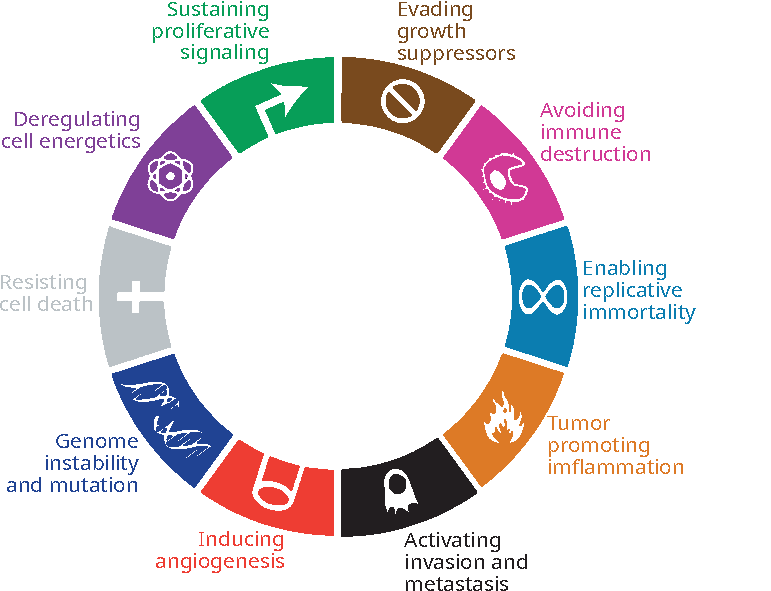
\includegraphics{CancerHallmarks.pdf}
			\caption[Cancer hallmarks]{The cancer hallmarks adapted from~\cite{Hanahan2011}}\label{fig:cancer_hallmarks}
		\end{figure}
		Despite being a group of more than a hundred different diseases, cancers share similar characteristics.
		These shared properties are known as the hallmarks of cancer and are defined as \textcquote{Hanahan2000,Hanahan2011}{acquired functional capabilities that allow cancer cells to survive, proliferate, and disseminate.}.
		They present an organizing principle to approach the complexity of cancers.
		The hallmarks define six capabilities: sustaining proliferative signaling, evading growth suppressors, activating evasion and metastasis, enabling replicative immortality, inducing angiogenesis and resisting cell death; two enabling capabilities: genome instability and mutation, and tumor-promoting inflammation; and two emerging hallmarks:deregulating cellular energetics and avoiding immune destruction.

\section{Omics data}
	The omics field corresponds to the characterization and quantification of pools of biological molecules.
	Each omics field studies an \emph{ome}.
	The \emph{ome} suffix refers to all constituents.
	For instance, the genome refers to all the genetic information of an organism, and genomics corresponds to the study of the genome.

	\begin{figure}[htbp]
		\centering
		\ifSubfilesClassLoaded{%
			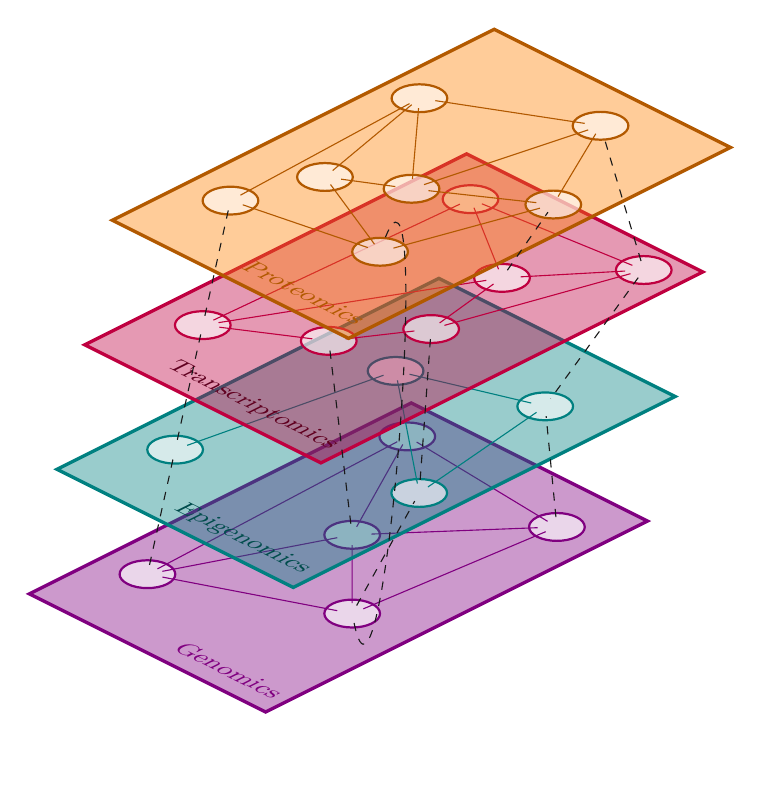
\begin{tikzpicture}
    \begin{scope}[
            yshift=0,
            yslant=-0.5,xslant=1,
            every node/.append style={yslant=-0.5,xslant=1}
        ]
        \fill[violet,fill opacity=0.4] (0,0) rectangle (3,4.85);
        \draw[violet,very thick] (0,0) rectangle (3,4.85);
        \draw[violet, thick, fill=white, fill opacity=0.6] (0.5,1) circle (2.5mm) node (G1) {};
        \draw[violet, thick, fill=white, fill opacity=0.6] (2.3,1.8) circle (2.5mm) node (G2) {};
        \draw[violet, thick, fill=white, fill opacity=0.6] (1.3,2.8) circle (2.5mm) node (G3) {};
        \draw[violet, thick, fill=white, fill opacity=0.6] (2.5,4.2) circle (2.5mm) node (G4) {};
        \draw[violet, thick, fill=white, fill opacity=0.6] (0.4,4.4) circle (2.5mm) node (G5) {};

        \node[anchor=east, font=\footnotesize, text=violet] at (3,0.3) {Genomics};
        \draw[violet] (G1) -- (G2);
        \draw[violet] (G1) -- (G3);
        \draw[violet] (G4) -- (G3);
        \draw[violet] (G2) -- (G4);
        \draw[violet] (G2) -- (G3);
        \draw[violet] (G3) -- (G5);
        \draw[violet] (G4) -- (G5);
        \draw[violet] (G1) -- (G5);
    \end{scope}

    \begin{scope}[
            yslant=-0.5,xslant=1,
            every node/.append style={yslant=-0.5,xslant=1},
            yshift=50, xshift=-40
        ]
        \fill[teal,fill opacity=0.4] (0,0) rectangle (3,4.85);
        \draw[teal,very thick] (0,0) rectangle (3,4.85);
        \draw[teal, thick, fill=white, fill opacity=0.6] (0.5,1) circle (2.5mm) node (E1) {};
        \draw[teal, thick, fill=white, fill opacity=0.6] (0.9,3.4) circle (2.5mm) node (E2) {};
        \draw[teal, thick, fill=white, fill opacity=0.6] (2.6,2) circle (2.5mm) node (E3) {};
        \draw[teal, thick, fill=white, fill opacity=0.6] (2.3,3.9) circle (2.5mm) node (E4) {};
        \node[anchor=east, font=\footnotesize, text=teal!60!black] at (3,0.3) {Epigenomics};

        \draw[teal] (E1) -- (E2);
        \draw[teal] (E4) -- (E2);
        \draw[teal] (E4) -- (E3);
        \draw[teal] (E2) -- (E3);

        \draw[black!90, dashed] (G1) -- (E1);
        \draw[black!90, dashed] (G4) -- (E4);
        \draw[black!90, dashed] (G2) -- (E3);
        %\draw[black!90, dashed] (G3) -- (E2);
    \end{scope}

    \begin{scope}[
            yslant=-0.5,xslant=1,
            every node/.append style={yslant=-0.5,xslant=1},
            yshift=100, xshift=-80
        ]
        \fill[purple,fill opacity=0.4] (0,0) rectangle (3,4.85);
        \draw[purple,very thick] (0,0) rectangle (3,4.85);
        \draw[purple, thick, fill=white, fill opacity=0.6] (0.5,1) circle (2.5mm) node (T1) {};
        \draw[purple, thick, fill=white, fill opacity=0.6] (0.6,4.3) circle (2.5mm) node (T2) {};
        \draw[purple, thick, fill=white, fill opacity=0.6] (2.6,4.5) circle (2.5mm) node (T3) {};
        \draw[purple, thick, fill=white, fill opacity=0.6] (2,2.4) circle (2.5mm) node (T4) {};
        \draw[purple, thick, fill=white, fill opacity=0.6] (1.5,1.6) circle (2.5mm) node (T5) {};
        \draw[purple, thick, fill=white, fill opacity=0.6] (1.8,3.5) circle (2.5mm) node (T6) {};
        \node[anchor=east, font=\footnotesize, text=purple!50!black] at (3,0.3) {Transcriptomics};

        \draw[purple] (T1) -- (T2);
        \draw[purple] (T1) -- (T5);
        \draw[purple] (T4) -- (T5);
        \draw[purple] (T4) -- (T6);
        \draw[purple] (T4) -- (T3);
        \draw[purple] (T3) -- (T6);
        \draw[purple] (T2) -- (T6);
        \draw[purple] (T2) -- (T3);
        \draw[purple] (T1) -- (T6);

        \draw[black!90, dashed] (T1) -- (E1);
        \draw[black!90, dashed] (T3) -- (E4);
        \draw[black!90, dashed] (T4) -- (E3);
        \draw[black!90, dashed] (T5) -- (G3);
    \end{scope}

    \begin{scope}[
            yslant=-0.5,xslant=1,
            every node/.append style={yslant=-0.5,xslant=1},
            yshift=150, xshift=-120
        ]
        \fill[orange,fill opacity=0.4] (0,0) rectangle (3,4.85);
        \draw[orange!70!black,very thick] (0,0) rectangle (3,4.85);
        \draw[orange!70!black, thick, fill=white, fill opacity=0.6] (0.5,1) circle (2.5mm) node (P1) {};
        \draw[orange!70!black, thick, fill=white, fill opacity=0.6] (0.8,1.9) circle (2.5mm) node (P2) {};
        \draw[orange!70!black, thick, fill=white, fill opacity=0.6] (0.4,3.5) circle (2.5mm) node (P3) {};
        \draw[orange!70!black, thick, fill=white, fill opacity=0.6] (2.6,3) circle (2.5mm) node (P4) {};
        \draw[orange!70!black, thick, fill=white, fill opacity=0.6] (1.9,4.3) circle (2.5mm) node (P5) {};
        \draw[orange!70!black, thick, fill=white, fill opacity=0.6] (1.5,2.3) circle (2.5mm) node (P6) {};
        \draw[orange!70!black, thick, fill=white, fill opacity=0.6] (2.1,1.3) circle (2.5mm) node (P7) {};

        \node[anchor=east, font=\footnotesize, text=orange!70!black] at (3,0.3) {Proteomics};
        \draw[orange!70!black] (P1) -- (P3);
        \draw[orange!70!black] (P3) -- (P5);
        \draw[orange!70!black] (P3) -- (P6);
        \draw[orange!70!black] (P6) -- (P5);
        \draw[orange!70!black] (P2) -- (P7);
        \draw[orange!70!black] (P4) -- (P5);
        \draw[orange!70!black] (P4) -- (P7);
        \draw[orange!70!black] (P1) -- (P7);
        \draw[orange!70!black] (P6) -- (P4);
        \draw[orange!70!black] (P6) -- (P2);
        \draw[orange!70!black] (P3) -- (P2);

        \draw[black!90, dashed] (T1) -- (P1);
        \draw[black!90, dashed] (T3) -- (P5);
        \draw[black!90, dashed] (T6) -- (P4);
        \draw[black!90, dashed] (G2) to [bend right=172] (P7);

    \end{scope}

\end{tikzpicture}%
		}{
			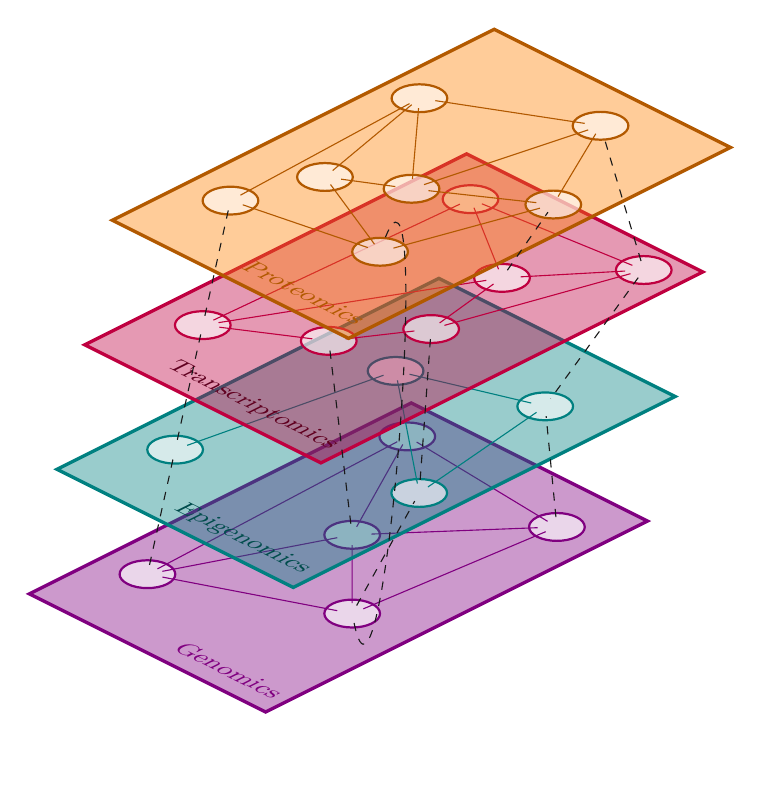
\begin{tikzpicture}
    \begin{scope}[
            yshift=0,
            yslant=-0.5,xslant=1,
            every node/.append style={yslant=-0.5,xslant=1}
        ]
        \fill[violet,fill opacity=0.4] (0,0) rectangle (3,4.85);
        \draw[violet,very thick] (0,0) rectangle (3,4.85);
        \draw[violet, thick, fill=white, fill opacity=0.6] (0.5,1) circle (2.5mm) node (G1) {};
        \draw[violet, thick, fill=white, fill opacity=0.6] (2.3,1.8) circle (2.5mm) node (G2) {};
        \draw[violet, thick, fill=white, fill opacity=0.6] (1.3,2.8) circle (2.5mm) node (G3) {};
        \draw[violet, thick, fill=white, fill opacity=0.6] (2.5,4.2) circle (2.5mm) node (G4) {};
        \draw[violet, thick, fill=white, fill opacity=0.6] (0.4,4.4) circle (2.5mm) node (G5) {};

        \node[anchor=east, font=\footnotesize, text=violet] at (3,0.3) {Genomics};
        \draw[violet] (G1) -- (G2);
        \draw[violet] (G1) -- (G3);
        \draw[violet] (G4) -- (G3);
        \draw[violet] (G2) -- (G4);
        \draw[violet] (G2) -- (G3);
        \draw[violet] (G3) -- (G5);
        \draw[violet] (G4) -- (G5);
        \draw[violet] (G1) -- (G5);
    \end{scope}

    \begin{scope}[
            yslant=-0.5,xslant=1,
            every node/.append style={yslant=-0.5,xslant=1},
            yshift=50, xshift=-40
        ]
        \fill[teal,fill opacity=0.4] (0,0) rectangle (3,4.85);
        \draw[teal,very thick] (0,0) rectangle (3,4.85);
        \draw[teal, thick, fill=white, fill opacity=0.6] (0.5,1) circle (2.5mm) node (E1) {};
        \draw[teal, thick, fill=white, fill opacity=0.6] (0.9,3.4) circle (2.5mm) node (E2) {};
        \draw[teal, thick, fill=white, fill opacity=0.6] (2.6,2) circle (2.5mm) node (E3) {};
        \draw[teal, thick, fill=white, fill opacity=0.6] (2.3,3.9) circle (2.5mm) node (E4) {};
        \node[anchor=east, font=\footnotesize, text=teal!60!black] at (3,0.3) {Epigenomics};

        \draw[teal] (E1) -- (E2);
        \draw[teal] (E4) -- (E2);
        \draw[teal] (E4) -- (E3);
        \draw[teal] (E2) -- (E3);

        \draw[black!90, dashed] (G1) -- (E1);
        \draw[black!90, dashed] (G4) -- (E4);
        \draw[black!90, dashed] (G2) -- (E3);
        %\draw[black!90, dashed] (G3) -- (E2);
    \end{scope}

    \begin{scope}[
            yslant=-0.5,xslant=1,
            every node/.append style={yslant=-0.5,xslant=1},
            yshift=100, xshift=-80
        ]
        \fill[purple,fill opacity=0.4] (0,0) rectangle (3,4.85);
        \draw[purple,very thick] (0,0) rectangle (3,4.85);
        \draw[purple, thick, fill=white, fill opacity=0.6] (0.5,1) circle (2.5mm) node (T1) {};
        \draw[purple, thick, fill=white, fill opacity=0.6] (0.6,4.3) circle (2.5mm) node (T2) {};
        \draw[purple, thick, fill=white, fill opacity=0.6] (2.6,4.5) circle (2.5mm) node (T3) {};
        \draw[purple, thick, fill=white, fill opacity=0.6] (2,2.4) circle (2.5mm) node (T4) {};
        \draw[purple, thick, fill=white, fill opacity=0.6] (1.5,1.6) circle (2.5mm) node (T5) {};
        \draw[purple, thick, fill=white, fill opacity=0.6] (1.8,3.5) circle (2.5mm) node (T6) {};
        \node[anchor=east, font=\footnotesize, text=purple!50!black] at (3,0.3) {Transcriptomics};

        \draw[purple] (T1) -- (T2);
        \draw[purple] (T1) -- (T5);
        \draw[purple] (T4) -- (T5);
        \draw[purple] (T4) -- (T6);
        \draw[purple] (T4) -- (T3);
        \draw[purple] (T3) -- (T6);
        \draw[purple] (T2) -- (T6);
        \draw[purple] (T2) -- (T3);
        \draw[purple] (T1) -- (T6);

        \draw[black!90, dashed] (T1) -- (E1);
        \draw[black!90, dashed] (T3) -- (E4);
        \draw[black!90, dashed] (T4) -- (E3);
        \draw[black!90, dashed] (T5) -- (G3);
    \end{scope}

    \begin{scope}[
            yslant=-0.5,xslant=1,
            every node/.append style={yslant=-0.5,xslant=1},
            yshift=150, xshift=-120
        ]
        \fill[orange,fill opacity=0.4] (0,0) rectangle (3,4.85);
        \draw[orange!70!black,very thick] (0,0) rectangle (3,4.85);
        \draw[orange!70!black, thick, fill=white, fill opacity=0.6] (0.5,1) circle (2.5mm) node (P1) {};
        \draw[orange!70!black, thick, fill=white, fill opacity=0.6] (0.8,1.9) circle (2.5mm) node (P2) {};
        \draw[orange!70!black, thick, fill=white, fill opacity=0.6] (0.4,3.5) circle (2.5mm) node (P3) {};
        \draw[orange!70!black, thick, fill=white, fill opacity=0.6] (2.6,3) circle (2.5mm) node (P4) {};
        \draw[orange!70!black, thick, fill=white, fill opacity=0.6] (1.9,4.3) circle (2.5mm) node (P5) {};
        \draw[orange!70!black, thick, fill=white, fill opacity=0.6] (1.5,2.3) circle (2.5mm) node (P6) {};
        \draw[orange!70!black, thick, fill=white, fill opacity=0.6] (2.1,1.3) circle (2.5mm) node (P7) {};

        \node[anchor=east, font=\footnotesize, text=orange!70!black] at (3,0.3) {Proteomics};
        \draw[orange!70!black] (P1) -- (P3);
        \draw[orange!70!black] (P3) -- (P5);
        \draw[orange!70!black] (P3) -- (P6);
        \draw[orange!70!black] (P6) -- (P5);
        \draw[orange!70!black] (P2) -- (P7);
        \draw[orange!70!black] (P4) -- (P5);
        \draw[orange!70!black] (P4) -- (P7);
        \draw[orange!70!black] (P1) -- (P7);
        \draw[orange!70!black] (P6) -- (P4);
        \draw[orange!70!black] (P6) -- (P2);
        \draw[orange!70!black] (P3) -- (P2);

        \draw[black!90, dashed] (T1) -- (P1);
        \draw[black!90, dashed] (T3) -- (P5);
        \draw[black!90, dashed] (T6) -- (P4);
        \draw[black!90, dashed] (G2) to [bend right=172] (P7);

    \end{scope}

\end{tikzpicture}%
		}
		\caption[Multi-omics layers]{Various layers of interconnected omics data. Connections between omics are represented by the black dashed links and connections between features in each omics are represented by the colored links.}\label{fig:multiomics_layers}
	\end{figure}

	The development of high-throughput technologies and the cost decline associated with those technologies helped foster a wide adoption of those methods.
	This adoption enabled a large availability of omics data, particularly multi-omics data, which helped revolutionize the field of precision medicine.
	There are multiple platforms to study omics data with different protocols, multiple references and annotations files, and various tools to perform the final quantification.
	This variability leads to highly heterogeneous data.
	Furthermore, omics data are complex data with many variables; for instance, transcriptomics has around 60K variables, and genomics and methylation data can exceed the hundreds of thousands of variables.

	In the following section, I will describe the main omics used in precision medicine and how they are obtained.

	\subsection{Genomics}\label{subsec:genomics}
		Genomics corresponds to the study of an organism's genome, \ie{}all its genetic information.
		The genetic information corresponds to the DNA sequence, which includes protein-coding genes, non-coding genes, and other regulatory elements.
		The DNA sequence is obtained with \gls{ngs} techniques.
		In the following, I will only describe Illumina sequencing, a sequencing-by-synthesis approach.
		After extracting and purifying the DNA of a sample, it is cut into small fragments of hundreds of base pairs to form the DNA library.
		Then, adapters are added to the fragments; the adapters contain a barcode to identify the sample, the binding site for the sequencing primer, and the complementary sequence to the oligonucleotides on the flow cell.
		The complementary sequence allows the fragment to attach to the flow cell during the sequencing.
		Each fragment is then amplified into distinct clonal clusters by bridge amplification.
		Sequencing is then performed using a cyclic process that adds fluorescent labeled nucleotides one at a time.
		A camera that captures the emitted fluorescence identifies the incorporated base at each position.
		The cycle is repeated numerous times to obtain completed DNA sequences: reads.
		After the sequencing, a set of reads is obtained, and those reads are aligned to a reference genome with an aligner.
		A variant calling step is then performed to identify single nucleotide variants.
		The variant calling step will quantify the different \gls{snp} in a DNA sequence; in other words, it will show the mutations that occur compared to the reference sequence.

		Quantification of \gls{cnv} is done with sequencing-based approaches or microarray.

	\subsection{Transcriptomics}\label{subsec:transcriptomics}
		Transcriptomics studies all RNAs transcript of an organism, \ie{}its transcriptome.
		The RNA is extracted from the sample, and messenger RNAs are enriched with a poly-A selection process.
		After fragmentation of the RNA molecule, a reverse transcriptase is used to convert the transcript into its \gls{cdna} sequence.
		The \gls{cdna} fragment is then sequenced as described in the \cref{subsec:genomics}.
		The reads are aligned to a reference genome; an annotation file is used to count the number of reads that map to a region known as a coding gene.
		The resulting count matrix can later be normalized to account for the sequencing depth and the gene length in \gls{fpkm}, \gls{tpm}, or any other normalization, depending on the study needs.

	\subsection{Epigenomics}
		Epigenomics is the study of the epigenome, the epigenetic modification of the genetic material.
		Epigenetic modification corresponds to a modification of a cell function: a gene regulation without any modification to the DNA sequence.
		Different mechanisms can produce such changes:
		\begin{itemize}[nosep]
			\item \glsxtrfull{dnam},
			\item histone modification,
			\item \glsxtrfull{mirna},
			\item \glsxtrfull{lncrna}.
		\end{itemize}

		\begin{figure}[htbp]
			\centering
			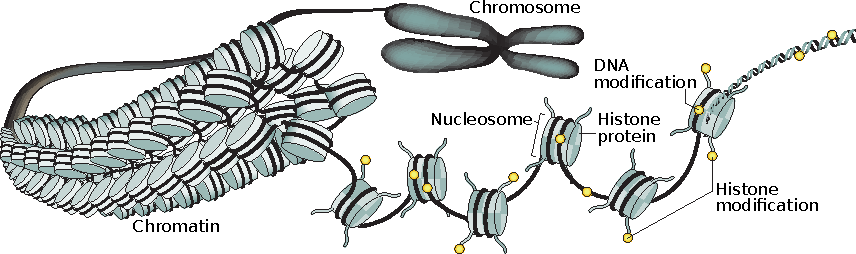
\includegraphics[width=\textwidth]{epigenetics.pdf}
			\caption[Epigenetic markers]{Epigenetics markers from~\cite{Jones2016}}\label{fig:epigenetics}
		\end{figure}

		\gls{mirna} and \gls{lncrna} quantification is obtained similarly to mRNAs quantification~(\cref{subsec:transcriptomics}).
		Histone modifications are quantified with a mass-spectrometry-based approach, see \cref{subsec:proteomics}.
		\Gls{dnam} is quantified with bead-chip-based methylation assay or bisulfite sequencing.
		The bisulfite treatment converts unmethylated cytosine into uracil.
		Then, the DNA sequence is sequenced as described in \cref{subsec:genomics}.
		A bisulfite treatment is also applied to the bead-chip assay.
		There are two types of beads for each targeted CpG on the plate.
		One of the beads corresponds to the methylated site, and the other to the unmethylated cytosine.
		After hybridization with the bead, a single base extension is performed with labeled nucleotides.
		The plate is then read to quantify the intensities of the methylated and unmethylated beads.
		For each CpG site, a ratio of the two intensities is computed, known as the \(\beta\) value.
		A value of one corresponds to a total methylation of the locus, and a value of zero to a total unmethylation of the locus.
		There are three different Illumina BeadChip methylation assays, each with a different coverage of the methylation sites in the human genome.
		The \(\beta\) values represent the methylation ratio at the locus level, and the methylation ratio at the gene level is computed as the average of all probes located within 1500 base pairs of a gene transcription start site.

	\subsection{Proteomics}\label{subsec:proteomics}
		Proteomics is the study of all proteins of an organism, also known as the proteome.
		Proteomics is more challenging to study; the DNA content of an organism is the same in all cells, whereas the protein content between two cells can strongly differ.
		This results from cell differentiation, where different genes are expressed in different cell types.
		Quantification of proteins can be achieved with an antibodies-based approach or antibody-free methods.
		One of the main antibody-based methods is \gls{rppa}, which allows for the simultaneous quantification of multiple proteins from multiple samples.
		Samples are immobilized on a solid support and probed with specific antibodies targeted to the proteins of interest.
		One antibody-free approach is based on mass-spectrometry; it is used to determine the amino acid sequence of a protein.
		Proteins are digested into smaller peptides; mass-to-charge ratios are measured with mass-spectrometry.
		The signal intensities reflect the quantity of peptides.
		Peptides mass-to-charge ratios are compared to theoretical ratios databases to identify the proteins.

\section{Datasets}
	Large multi-omics datasets are limited, and although the cost of high\-/throughput technologies has decreased, many difficulties remain in the acquisition of multi-omics data.
	\Gls{tcga} is the main dataset with high-quality patient data~\cite{TCGA}, \gls{ccle} is another multi-omics dataset on cell-lines~\cite{CCLE}.
	Those datasets present uniformly processed data, ensuring that samples were analyzed the same way.

	\subsection{\Glsfmtfull{tcga}}\label{sec:data_tcga}
		Among the 33 cancer types available in the \gls{tcga} project, we selected 19 cancers with more than a hundred patients.
		We collected a total of 8777 samples, 8416 were cancer samples and 361 normal samples from the GDC Data Portal\footnote{\url{https://portal.gdc.cancer.gov/}} with the \textsf{TCGABiolinks} R package.
		For all selected patients we collected, when available, \glsxtrfull{dnam}, \glsxtrfull{mrna}, \glsxtrfull{mirna} expression, \glsxtrfull{cnv}, and proteomics.
		Clinical annotations are also available for each patient.
		In \gls{tcga}, cancerous samples encompass primary solid tumor, recurrent solid tumor, and metastasis.
		The normal samples correspond to solid tissue; a portion of tissue is sampled at a certain distance from the tumor or are blood-derived.
		Multiple predictive endpoints are available in \gls{tcga}:
		\begin{itemize}[nosep]
			\item type of sample (binary classification),
			\item type of cancer (multiclass classification),
			\item cancer subtype (multiclass classification),
			\item metastasis origin (multiclass classification),
			\item cancer stage (multiclass classification),
			\item primary diagnosis (multiclass classification),
			\item disease type (multiclass classification),
			\item survival (risk prediction or survival time prediction).
		\end{itemize}
		This non-exhaustive list shows the diversity of available tasks in \gls{tcga}, making it a well-studied dataset.
		When using the cancer stage as predictive endpoints, it is important to note that in \gls{tcga}, patients with the same stage might not share the same properties.
		Indeed, the cancer staging criteria differ between cancers, and those criteria evolve over time as new staging classifications are regularly published.

		% https://www.ncbi.nlm.nih.gov/pmc/articles/PMC8368987/
		%primary origin of a metastasis % https://www.nature.com/articles/s41467-019-13825-8
		%predict primary or metastasis % https://www.frontiersin.org/articles/10.3389/fmolb.2022.913602/full
		% https://www.nature.com/articles/s41598-023-35842-w


		All samples in \gls{tcga} are processed in an harmonized way\footnote{\url{https://gdc.cancer.gov/about-data/gdc-data-processing}} against common reference files\footnote{\url{https://gdc.cancer.gov/about-data/gdc-data-processing/gdc-reference-files}}.
		According to the \gls{tcga} consortium recommendation, we removed FFPE samples as they are not suitable for molecular analysis\footnote{\href{https://web.archive.org/web/20150919082952/https://gdac.broadinstitute.org/runs/sampleReports/latest/FPPP_FFPE_Cases.html}{\nolinkurl{https://gdac.broadinstitute.org/runs/sampleReports/latest/FPPP\_FFPE\_Cases.html}}}.
		We also followed their recommendation to select the best replicate\footnote{\href{https://web.archive.org/web/20150919044554/http://gdac.broadinstitute.org/runs/sampleReports/latest/READ_Replicate_Samples.html}{\nolinkurl{https://gdac.broadinstitute.org/runs/sampleReports/latest/READ\_Replicate\_Samples.html}}}.
		In \gls{tcga}, \gls{dnam} data is collected with two different methods: Illumina Human Methylation 450 and Human Methylation 27.
		The methylation 450 platform contains more CpG sites but contains 94\% of the CpG sites detected by the methylation 27 method.
		\Gls{dnam} data was restricted to the probes common to both HumanMethylation27 and HumanMethylation450 platforms.
		A total of 8416 patients of 19 different cancers and 361 normal samples were collected.
		Features with more than 10\% of NaN values were removed, remaining NaN were imputed using \gls{knn} imputation.
		No feature selection was applied, and data were standardized to a zero mean and unit variance.
		Patients with incorrect survival information were removed, leaving 8349 patients for survival prediction.

		For the multi-omics study, we restricted the dataset to patients having all modalities present, which led us to select 5862 patients of 18 different cancers.
		This selection process ensures that the dataset only contains paired data.
		We also considered coding and \gls{ncrna} as two different modalities, as \gls{ncrna} can affect cancer cell fate through various mechanisms~\cite{Grillone2020} and are involved in the oncogenesis~\cite{Toden2021}.
		In this manuscript, we focused on two tasks: cancer-type prediction and risk-based survival prediction.
		70\% of the data was used as a training set, 15\% forms the validation set, and the remaining 15\% forms the test set while preserving the proportion of each cancer.
		The training set is used to train the different models, the validation set is used to select the best model hyperparameters, and the test set is used to assess the model performances.

	\subsection{\Glsfmtfull{ccle}}\label{sec:data_ccle}
		This second dataset, available on the DepMap portal\footnote{\url{https://depmap.org/portal/data_page/?tab=allData}}, is composed of \glsxtrfull{dnam}, \glsxtrfull{mrna}, \glsxtrfull{mirna} expression, \glsxtrfull{cnv}, metabolomics, and proteomics for 536 cells of 16 different cancers.
		Methods to obtain the molecular features from the cancer cell-lines is described in~\cite{CCLE}.
		Contrary to \gls{tcga}, \gls{dnam} data were quantified with reduced representation bisulfite sequencing which focuses on methylation sites in promoters regions.
		No feature selection was applied, and data were standardized to a zero mean and unit variance.
		70\% of the data was used as a training set, 15\% forms the validation set, and the remaining 15\% forms the test set while preserving the proportion of each cancer.

\end{document}
